\newpage
\begin{center}
  \textbf{\large 2. ТЕХНИЧЕСКАЯ РЕАЛИЗАЦИЯ}
\end{center}
\refstepcounter{chapter}
\addcontentsline{toc}{chapter}{2. ТЕХНИЧЕСКАЯ РЕАЛИЗАЦИЯ}

\section{Описание бизнес-процессов} 

Главные процессы связаны с выполнением вычислительных задач и развертыванием контейнеров, что требует ручной настройки серверной инфраструктуры и управления вычислительными ресурсами. Это обеспечивает выполнение клиентских запросов, но сопровождается значительными временными затратами и сложностями администрирования. На рисунке ~\ref{IDEF0_AS-IS} показан сам бизнес-процесс выполнения вычислительных задач и развертывания контейнеров до автоматизации, а на рисунке ~\ref{IDEF0_AS-IS_Extended} представлена декомпозиция данного процесса.

\begin{figure*}[!t] 
  \centering
  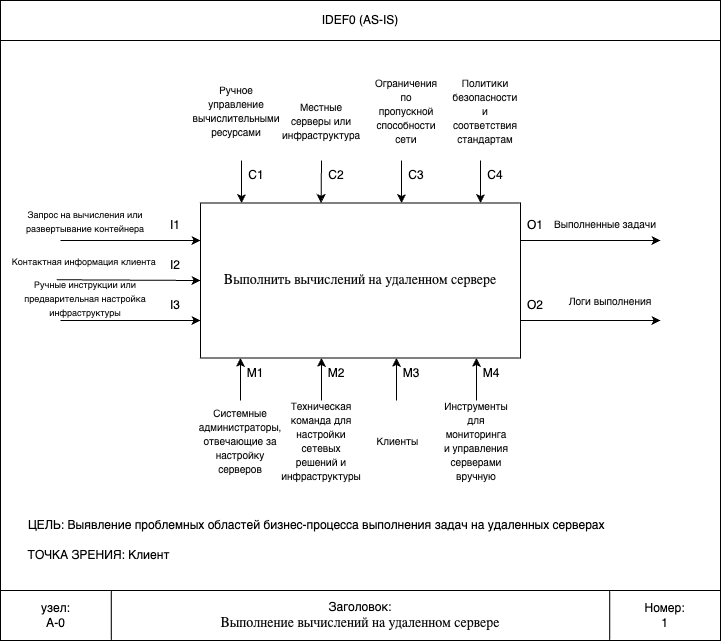
\includegraphics[width=\linewidth]{generated/IDEF0_AS-IS.drawio.png}
  \caption{Процесс выполнения вычислений на удаленном сервере}
  \label{IDEF0_AS-IS}
\end{figure*}

Среди основных проблем неавтоматизированного бизнес-процесса можно выделить:
\begin{itemize}
  \item[---]получение запросов от клиентов через ручные каналы связи, что увеличивает время на их обработку и уточнение технических требований;
  \item[---]ручное конфигурирование серверной инфраструктуры под каждую задачу, что требует значительных временных и трудовых затрат от администраторов;
  \item[---]отсутствие централизованной системы мониторинга выполнения задач, что приводит к необходимости постоянного ручного контроля и увеличению вероятности ошибок;
  \item[---]передача результатов клиентам осуществляется вручную, что замедляет процесс и увеличивает вероятность задержек.
\end{itemize}

\begin{figure*}[!t]
  \centering
  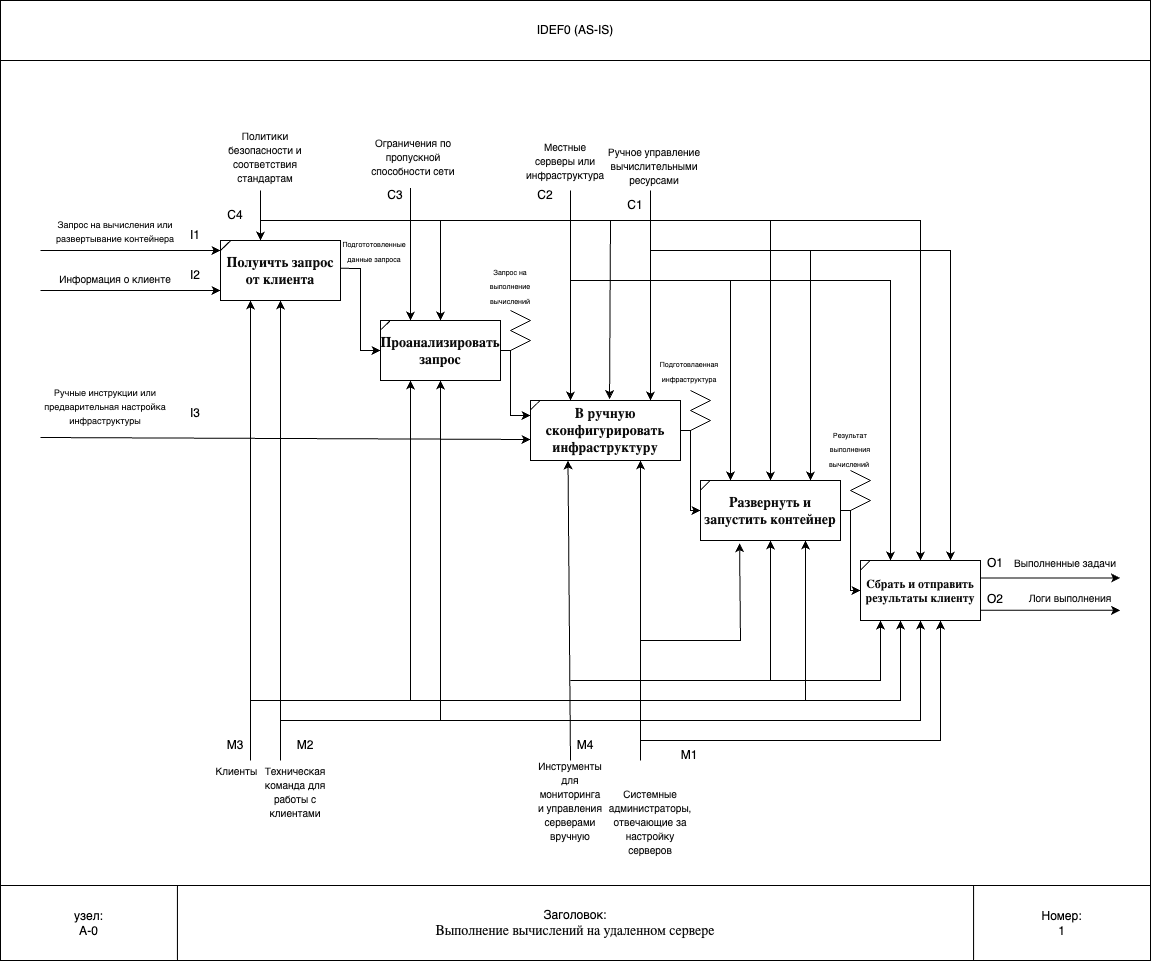
\includegraphics[width=\linewidth]{generated/IDEF0_AS-IS_Extended.drawio.png}
  \caption{Декомпозиция процесса выполения удаленных вычислений}
  \label{IDEF0_AS-IS_Extended}
\end{figure*}

После автоматизации значительно минимизируется участие специалистов в ручной настройке серверной инфраструктуры и мониторинге выполнения задач, что упрощает и ускоряет процесс развертывания и выполнения контейнеров. На рисунке ~\ref{IDEF0_TO-BE} показан бизнес-процесс выполнения лямбда-функций после автоматизации, а на рисунке ~\ref{IDEF0_TO-BE_Extended} представлена декомпозиция данного процесса.

\begin{figure*}[!t]
  \centering
  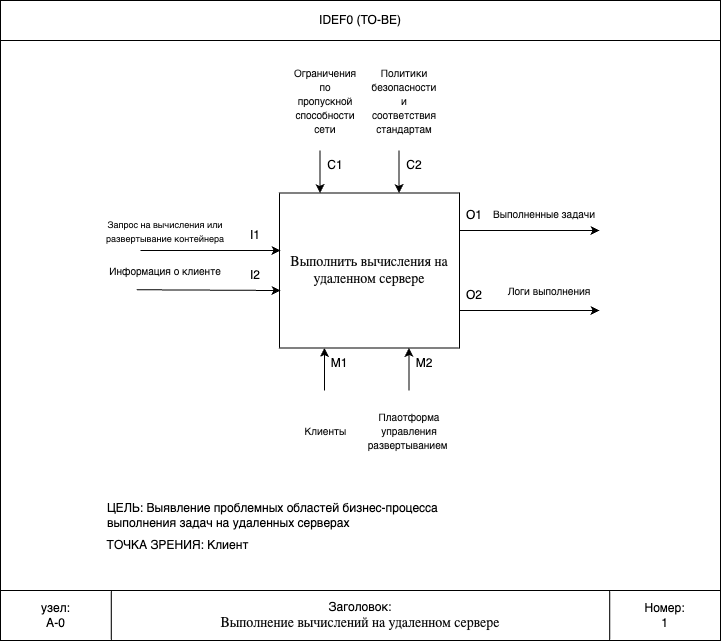
\includegraphics[width=\linewidth]{generated/IDEF0_TO-BE.drawio.png}
  \caption{Процесс выполнения вычислений в бессерверной среде}
  \label{IDEF0_TO-BE}
\end{figure*}

Основными преимуществами автоматизированного бизнес-процесса являются:
\begin{itemize}
  \item[---]автоматическое развертывание контейнеров с минимальным участием специалистов;
  \item[---]гибкость настройки выполнения задач благодаря удобному интерфейсу и API;
  \item[---]автоматическое формирование отчетов по выполнению задач и сбор статистики о загрузке ресурсов;
  \item[---]возможность одновременного выполнения множества задач с оптимизацией использования инфраструктуры.
\end{itemize}

\begin{figure*}[!t]
  \centering
  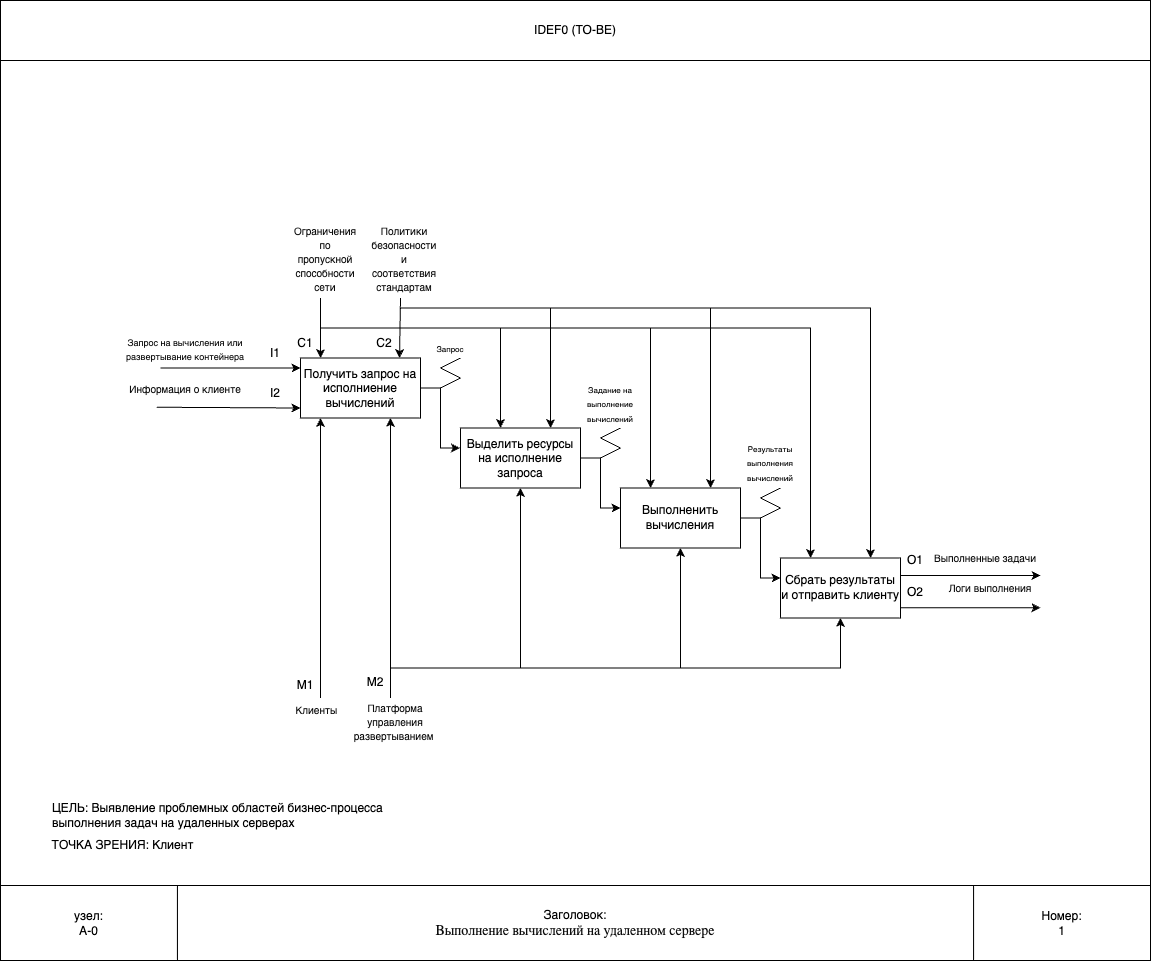
\includegraphics[width=\linewidth]{generated/IDEF0_TO-BE_Extended.drawio.png}
  \caption{Декомпозиция процесса выполения вычислений в бессерверверной среде}
  \label{IDEF0_TO-BE_Extended}
\end{figure*}

\section{Описание архитектуры решения}

Описание архитектуры приложения является ключевым этапом в проектировании програмного решения. Описанная архитектура позволяет разделить систему на независимые компоненты, определить взаимосвязи между ними, правила их мастабирования а так же обеспечить согласованность в их разработке. 

Разрабатываемое приложение представляет собой моногокомпонентное клиент-серверное решение и стоит незавыисимых функциональных блоков:

\begin{itemize}
  \item[---] Серверверная часть приложения
  \item[---] Клиентская часть приложения 
\end{itemize}

Серверная часть в свою очередь состоит из таких компонентов как:

\begin{itemize}
  \item[---] Reverse proxy\cite{sommerlad2003reverse};
  \item[---] Internal API Gateway
  \item[---] External API Gateway
  \item[---] Сревер авторизации
  \item[---] Брокер сообщений
  \item[---] СУБД
  \item[---] Слой платформенных сервисов
  \item[---] Подчиненный кластер Kubernetes
\end{itemize}

На рисунке ~\ref{SystemDiagram} представлена схема взаимодействия и размещения компонентов системы.

\begin{figure*}[!t]
  \centering
  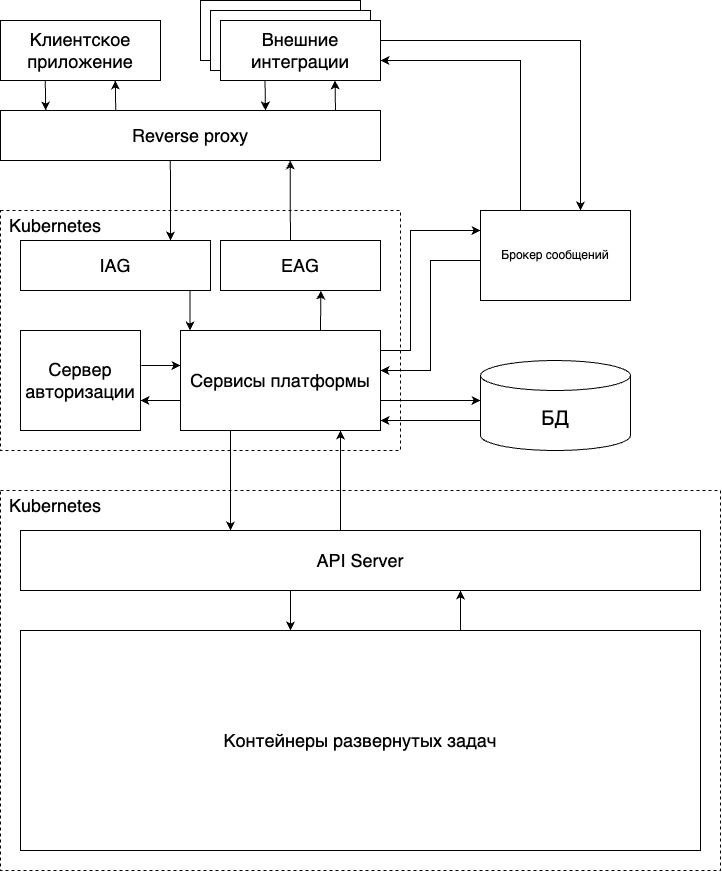
\includegraphics[width=\linewidth]{generated/SystemDiagram.drawio.png}
  \caption{Компоненты плфтормы}
  \label{SystemDiagram}
\end{figure*}

\subsection{Среда развертывания}

Сейчас на рынке существует несколько подходов к развертыванию сервисов. Каждая из представленных сред имеет свои плюсы и минусы.

\subsubsection{Физические серверы}

В настоящее время развертывание веб-сервисов на физических серверах является устаревшим подходом. Такой подход имеет большое число минусов, таких как необходимость управления зависимостями разворачиваемых сервосов, сложности с масштабированием.

\subsubsection{Виртуальные машины}

Вируальные машины позволяют запускать сервисы в изолированных вируальных средах, хорошо масштабируются но требуют ручного управления ресурсами, сильно уступают контейнерным решениям по эффективности использования ресусов и чаще всего исопльзуются для узкоспециализироанных сервисов.

\subsubsection{Контейнеры без оркестрации}

Развертывание в контейнерах без оркестрации хорошо подходит для разворачивания небольших сервисов а так же для локального запуска, но при использовании в промышленных средах требование ручного управления контейнерами делает такие системы неприменимыми.

\subsubsection{Контейнерные оркестраторы}

Контейнерные оркестраторы предоставляют возможность объединения нескольких физических серверов в один кластер с едиными ресурсами, таким образом осуществляется удиное эффективное управление всеми ресурсами системы, достигается ее масштабируемость и отказоустойчивость. 

\subsubsection{Выбор оркестратора}

Для разворачивания разрабатываемой платформы оптимальным выбором является Kubernets, так как он обеспечивает гибкое и эффективное управление ресурсами клстера при помощи yaml манифестов и является стандартом в индустрии для выполнения задач оркестрации контейнеров.

\subsection{Reverse proxy}

Размещение веб-сервера или сервера приложений непосредственно в Интернете дает злоумышленникам прямой доступ к любым уязвимостям базовой платформы (приложения, веб-сервера, библиотек, операционной системы). Для того что бы избежать появления такого рода уязвимостей широко распространен паттер Reverse-proxy\cite{sommerlad2003reverse}.

Reverse-proxy представляет собой промежуточный слой между внутренними сервисами приложения и внешними клиентами.
Так же веб-сервер, выступающий в роли reverse-proxy может выолнять следующие функции:

\begin{itemize}
  \item[---] Маршрутизация запросов;
  \item[---] Балансировка нагрузки;
  \item[---] SSl-терминация;
  \item[---] Фильтрация запросов;
  \item[---] Кеширование;
  \item[---] Сжатие контента;
  \item[---] Управление статическими ресурсами. 
\end{itemize}

В качестве reverse-proxy для реализации платформы был выбран веб-сервер nginx. Этот компонент будет отвечать за SSL-терминацию и раздачу статического контента.

\subsection{Ingress, Egress}

В качестве реализацией для Internal Api Gateway(IAG) и External Api Gateway(EAG) выбраны соотвествующие реализации Istio Ingress и Egress.

Главная задача которую выполняет IAG - распределение входящего трафика по репликам сервисов для обеспечения равномерного и эффективного использования ресурсов.

В то же время EAG отвечает за маршрутизацию исходящего трафика. Он служит точкой выхода трафика, направленного на получение внешних ресурсов.

\subsection{Сревер авторизации}

Сервер авторизации в плфторме отвечает за авторизацию и аутентификацию пользователей, а так же запросов от входящих интеграций, выполняет централизованное управление доступом к сервисам платформы. 

К возможным реализациям сервера авторизации можно отнести такие сервисы как:

Среди бошаого колличества реализаций сервера авторизации для платформы выбран сервис Keycloak. Keycloak по сравнению с конкурентами обладает следующими преимуществами:

\begin{itemize}
  \item[---] Решение с открытым исходным кодом;
  \item[---] Поддержка большого колличество протоколов авторизации и SSO;
  \item[---] Наличие системы управления польователями и ролями;
  \item[---] Нативная интеграция с Kubernetes и масштабируемость;
  \item[---] Возможность локального развертывания;
  \item[---] Подержка СУБД PostgresSQL;
  \item[---] Наличие Java клиента;
  \item[---] Наличие адаптера Spring Sequrity;
  \item[---] Наличие административной панели. 
\end{itemize}

\subsection{Брокер сообщений}

Брокер сообщений это промежуточное звено в системе. Он обеспечивает асинхронное возаимодействие между компонентами системы. Основаная задача которую выполняет брокер сообщений - позволяет не дожидаться выполнения ресурсоемких операций и получить результат их выполнения асинхронно позже. 

Брокеры сообщений играют ключевую роль в реализации таких системных паттернов как очередь сообщений\cite{raje2019performance}, Saga\cite{durr2021evaluation}, а так же целого семейства Enterprise Integration Pattern (EIP)\cite{hohpe2004enterprise}.

На данный момент основными реализациями брокера сообщений представленными на рынке являются:

\begin{itemize}
  \item[---] Apache Kafka;
  \item[---] RabbitMQ;
  \item[---] ActiveMQ;
  \item[---] Redis Streams.
\end{itemize}

В качестве основого брокера сообщений на платформе выбран брокер сообщений Apache Kafka.
К основным плюсам по сравнению с другими реализациями брокеров можно отнести концептуальное отличие данного брокера отдругих представленным на рынке.

Kafka поррерживает многокартное потребление сообщений, делая возможными сценарии использования Kafka в качестве Enterprise Service Bus\cite{menge2007enterprise} и позволяет не терять сообщения при ошибках и прерываниях обработки.

Так же в преимуществам выбора брокера сообщений Kafka можно отнести:

\begin{itemize}
  \item[---] Масштабируемость и производительность;
  \item[---] Высокая доступность и отказоустойчивость;
  \item[---] Поддержка потоковой обработки;
  \item[---] Гибкость интеграции;
  \item[---] Интеграция с Kubernetes;
  \item[---] Обширная экосистема и поддержка сообщества.
\end{itemize}

\subsection{СУБД}

В проектируемой системе база данных неодходима для хранения у управления пользовательскими данными. Система управления базой данных(СУБД) обеспечивает эффективную организацию данных, в отдельных случаях транзакционность, целостность и надежность. СУБД так же предоставляет возможности масштабирования и интеграций с другими системами.

Все СУБД можно разделить на две группы по способу организации данных - реляционные и нереляционные. Главное отличие реляционных баз данных от нереляционных заключается в использовании реляционными базами данных таблиц с фиксированной схемой для хранения данных и поддержка строгих отношений между таблицами с использованием внешних ключей, в то время как нереляционные базы данных являются более гибкими и хранят данные в формате ключ - занчение и не продъявля/т каких либо требований к схеме хранимых данных.

Данные, хранимые платформой сильно структурированы и для выполнения бизнесс логики приложения критична их целостность, поэтому единственным верным выбором будет реляционная СУБД. На данный момент на рынке представлены следующие сервисы:

\begin{itemize}
  \item[---] PostgreSQL;
  \item[---] MySQL;
  \item[---] Oracle Database;
  \item[---] MariaDB.
\end{itemize}

Для исполновании в реализации платформы выбрана СУБД PostgreSQL по следующим причинам:

\begin{itemize}
  \item[---] Поддержка сложных типов данных, возможность расширения встроенных типов данных;
  \item[---] Поддержка транзакций;
  \item[---] Открытый исходный код и активное сообщество;
  \item[---] Масштабируемость и отказоустойчивость.
\end{itemize}

\subsection{Слой платформенных сервисов}

Слой платформенных сервисов играет ключевую роль в системе, так как именно он отвечает за функциональные возможности системы, управление процессами выполнения вычислений.

На данный момент существует два конкурируюзих подхода к организации сервсов приложений - монолит и микросервисы\cite{newman2019monolith}.

\subsubsection{Монолитная архитектура}

Монолитный сервис(Рис. ~\ref{monolith}) представляет собой единую единицу развертывания которая отвечает за все функции системы. При использовании такого подхода на начальных этапах можно добиться быстрого вывода на рынок основного функционала, но при длительной разработке и с использованием монолитной архтектуры можно столкнуться с проблемами со сложностью внесения изменений, увеличеии времени холодного старта, увеличением времени проходжения конвеера доставки и развертывания а так же с увеличенным расходом ресурсов при масштабировании и возможными периоднами недоступности при развертыании или неожданных отказах.

\begin{figure*}[!t]
  \centering
  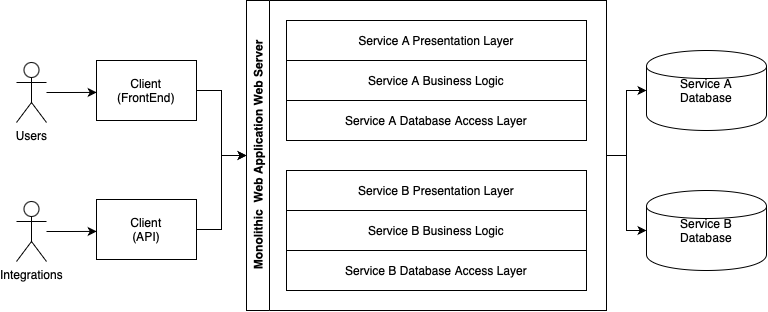
\includegraphics[width=\linewidth]{generated/monolith.drawio.png}
  \caption{Приложение с монолитной архитектурой}
  \label{monolith}
\end{figure*}

\subsubsection{Микросервисная архитектура}

Главная идея микросервисной архитектуры(Рис. ~\ref{microservice}) заключается в разделении системы на отдельные независимые подсистемы - микросервисы. Каждый микросервис должен отвечать за свою небольшую часть функционала.

Основыным преимуществом использования микросервисов является возможность независимого развертывания и прохожения конвеера доставки и развертывания. Микросервысы могут масштабироваться независимо, позваоля добавлять реплики нагруженным сервисам во время пиковых перидов нагрузки, а малонагруженные сервисы разворачивать с малым колличеством реплик.

\begin{figure*}[!t]
  \centering
  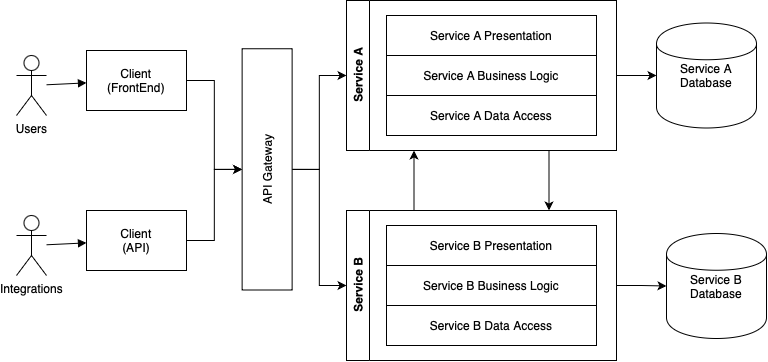
\includegraphics[width=\linewidth]{generated/microservice.drawio.png}
  \caption{Приложение с микросервисной архитектурой}
  \label{microservice}
\end{figure*}

Использование микросервисной архитектуры усложняет внесение изменений в существующую систему, а так же требует более сложного управления инфраструктурой.
При использовании микросервисной архитектуры появляется необхзодимость в сохранении обратной совместимости между версиями сервисов, так как при установке поставки на стенде может находиться одновременно старая и новая версия сервиса для поддржки плавной незамтной для пользователя раскатки.
Использвоание микросервисосв так же увеличивает время отклика сервисов, так как возникают дополнительные накладные расходы при выполнении межсервисных вызовов, так же при отказе отдельных сервисов могут возникат тредности с локализацией проблемы, что приводит к необзодимости внедрения распределенный трассировки вызовов.

\subsubsection{Выбор архитектуры сервисного слоя}

Для сервисного слоя платформы выбрана  монолитная архитектура, при этом необходимо осуществлять проектирование функционала так, что бы в последствие он мог быть отделен в отдельные сервисы. При разработке важно соблюдать слабую связанность\cite{valipour2009brief} между сервисами, используя такие подходы как Domain Driven Design(DDD) \cite{evans2004domain} или Verical Slice\cite{ratner2011vertical}

\subsection{Подчиненный кластер Kubernetes}

Подчиненный кластер Kubernetes в системе предназначен для разворачивания в нем задач, создаваемых пользователями. Он является выделенной изолированный средой которая обеспечивает гибкость, масштабируемость и отказоустойчивость системы.

\section{Обоснование технологического стека}

\subsection{Клиенская часть}

При разработке клиенской части приложения использован fontend фреймворк Vue3.
Для управления состоянием клиентского приложения испольована библиотука Pinia.
Для работы со стилизаций компонентов интерфейса использованы библиотки TailwindCSS и DaisyUI.

Такой стек технологий позволяет эффективно выполнять задачи, поставленные перед разработкой клиентской части.
Фреймворк Vue3 обладает полее высокой производительностью по сравнению с предыдущей версией Vue2 и аналогами React и Angurlar.

Так же Vue3 более удобен для разработки и имеет более низкий порог вхождения. Поддрежка TypeScript позволят разрабатывать более надежные и предсказуемые компоненты.

Менеджер управления состоянием приложения Pinia выбран так как является официальной заменой Vuex в Vue3. По сравнению с предшественником новый стейтменеджер более простой и понятный так как в нет мутаций и он по умолчанию поддерживает реактивность, которая пришла на смену CompositionAPI в новой версии фреймворка.

TailwindCSS это библиотека позволяюзая избежать работы со стилями компонентов напрямую. Благодаря гибкой системе заранее предопределенных классов библиотека позволяет сократить дублирование кода и ускорить разработку.

DaisyUI является самой большой и популярной библиотекой UI компонентов постоенной на TailwindCSS. Она предлагает большой набор компонентов и тем для приложения которые гибко интегрируются с остальной системой по средствам применения классов к HTML-тегам.

\subsection{Серверная часть}

Для разработки серверной части платформы выбран язые программиования Kotlin, этот язык относится к семейству языков компилирующихся в байткод поддерживаемый виртуальной машиной Java. Для разработки так же выбрана версия Java 21 так как она является самой последней версией языка для которой на момент написания работы заявлена длинтельня поддержка (LTS).

По сравнению с Java, Kotlin имеет более выразительный синтаксис и является более безопасным так как частью языка являются механимзмы защиты от разименования $null$ указателей\cite{samuel2017programming}.

Фреймворком для написания серверной чати приложения выбран Spring и Spring Boot.
Данное решение является стандартом в отрасти и зарекомандовало как себя удобное и эффективное для построения такого рода систем.

Экосистема Spring обладает большим колличеством библиотек позволяющими расширить функционал фемворка и интегрироваться с большинством сторонних систем.
Для разработки серверной части платформы с состав дистрибутива были включены следующие библиотеки:

\begin{itemize}
  \item[---] keycloak-admin-client --- для интеграции системы с сервером авторизации Keycloak через REST API;
  \item[---] spring-data-jdbc --- для интеграции с СУБД PostgreSQL;
  \item[---] kubernetes-client-java --- для интеграции системы с подчиненным кластером Kubernetes;
  \item[---] spring-security --- для обработки авторизационных токенов и создание политик доступа к предоставляемым сервисам.
\end{itemize}

Для сборки серверной касти приложения выбрана система автоматической сборки Gradle, так как она является современной заменой устаревший системе сборки Maven, дает более гибкий и удобный инструментарий, а так же на момент написания работы является стандартом в отрасли. 

\section{Разработка модели данных}

На платформе используется две базы данных - одна из них используется для хранения данных проектируемого сервиса, вторая - для хранения данных сервера авторизации.

\subsection{Модель базы данных сервиса}

В рамках предметной области основными сущностями являются пользователь, группа пользователей задача, результат выполнения задачи.

На рисунке ~\ref{DatabaseDiagram} ER диаграмма, на которой изображены сущности базы данных и взаимосвязи между ними.

\begin{figure*}[!t]
  \centering
  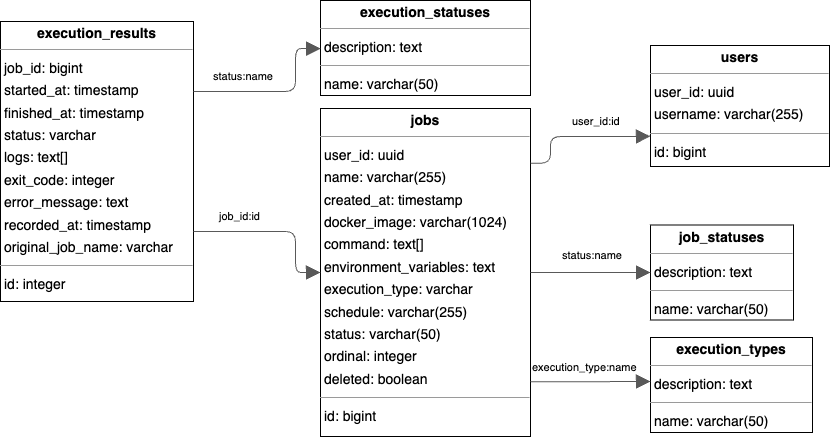
\includegraphics[width=\linewidth]{generated/database-diagram.png}
  \caption{Диаграмма отношений таблиц базы данных}
  \label{DatabaseDiagram}
\end{figure*}

В модели базы данных испльзуется подход по реализации перечислений (enumirations) с использованием референсных таблиц, в которых первичным ключом является колонка $name$, на которую ссылаются таблицы исполуьзующие значения из данной таблицы в качестве перечислений.
Колонка $description$ при этом является справочной и служит только для хранения человекочитаемого описания значения перечисления.

К референсным относятся таблицы $job\_statuses$, $execution\_statuses$, \linebreak $execution\_types$ которые хранят статусы задач и запусков.

Таблица $jobs$ является центральной таблицу для хранения информации о запущенных задачах. Статусом задачи является одно из значений поля $name$ референсной таблицы $job\_statuses$.
Время создания записи в таблицу фиксирутся автоматически а поле $created\_at$.

Таблица $jobs$ имеет сдедующие поля:

\begin{itemize}
  \item[---]$id$ --- $bigint$ — Уникальный идентификатор задачи.
  \item[---]$user\_id$ --- $uuid$ —-- Идентификатор пользователя, создавшего задачу.
  \item[---]$name$ --- $varchar(255)$ — Имя задачи.
  \item[---]$created\_at$ --- $timestamp$ — Время создания задачи.
  \item[---]$docker_image$ --- $varchar(1024)$ — Docker-образ, который используется для выполнения задачи.
  \item[---]$command$ --- $text$ — Команда или скрипт, который выполняется в рамках задачи.
  \item[---]$environment_variables$ --- $text$ — Переменные окружения, используемые для выполнения задачи.
  \item[---]$execution_type$ --- $varchar$ — Тип выполнения задачи;
  \item[---]$schedule$ --- $varchar(255)$ — Расписание выполнения задачи (cron-выражение).
  \item[---]$status$ --- $varchar(50)$ — Статус задачи.
  \item[---]$ordinal$ --- $integer$ — Порядковый номер задачи.
  \item[---]$deleted$ --- $boolean$ — Флаг, показывающий, удалена ли задача.
\end{itemize}

Результаты выполнения задач располагаются в таблице $execution\_result$. Для создания отношения один ко многим с таблицей $job\_statuses$, внешним ключем является поле $job\_id$.

Таблица $execution\_result$ имеет сдедующие поля:

\begin{itemize}
  \item[---]$id$ --- $integer$ — Уникальный идентификатор результата выполнения.
  \item[---]$job\_id$ --- $bigint$ — Идентификатор задачи, к которой привязан результат. 
  \item[---]$started\_at$ --- $timestamp$ — Время начала выполнения задачи.
  \item[---]$finished\_at$ --- $timestamp$ — Время завершения задачи.
  \item[---]$status$ --- $varchar$ — Статус выполнения задачи.
  \item[---]$logs$ --- $text$ — Массив логов, связанных с выполнением задачи.
  \item[---]$exit\_code$ --- $integer$ — Код завершения выполнения задачи.
  \item[---]$error\_message$ --- $text$ — Сообщение об ошибке.
  \item[---]$recorded_at$ --- $timestamp$ — Время записи результата выполнения.
  \item[---]$original\_job\_name$ --- $varchar$ — Оригинальное имя задачи.
\end{itemize}

Таблица $users$ хранит данные дублирующие информацию о зарегистрированных пользователях, хранящаюся на сервере авторизации. Она необходима для содния внешних ключей в которых значением является идентификатор пользователя в системе авторизации.

\subsection{Модель базы данных сервера авторизации}

Модель базы данных сервера авторизации играет важную роль в работе системы, так как информация о пользователях, а так же их положение в ролевой модели хранится на сервере авторизации.

Ключевыми сущностями хранения информации о пользователях являются пользователь, атрибут пользователя, группа, роль. ER диаграмма чати сервера авторизации по работе с данными пользователей и ролевой моделью представлена на рисунке ~\ref{KeyclaokDatabaseDiagram}.

\begin{figure*}[!t]
  \centering
  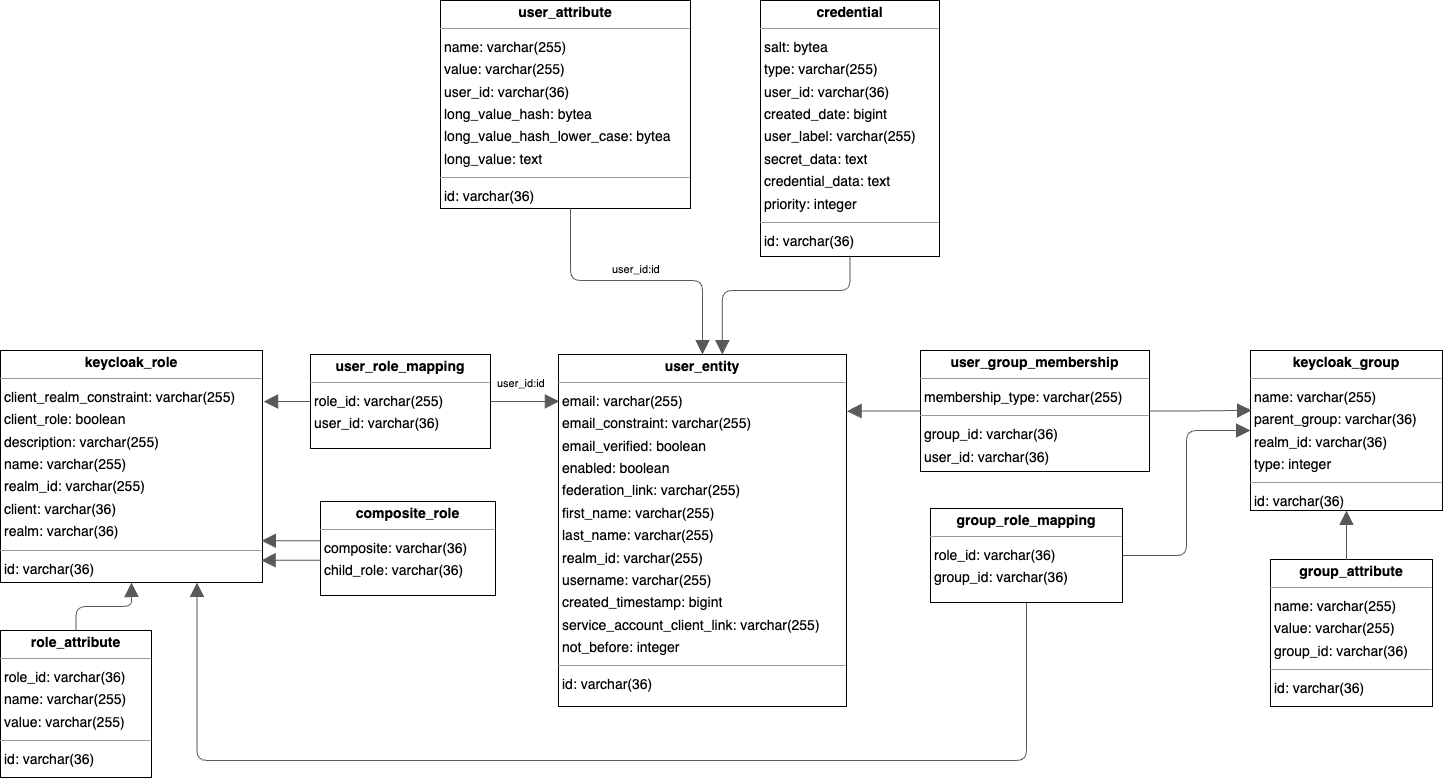
\includegraphics[width=\linewidth]{generated/keycloak-user-information-database-diagram.drawio.png}
  \caption{Модель хранения данных пользователей на сервере авторизации}
  \label{KeyclaokDatabaseDiagram}
\end{figure*}

Таблица $user\_entity$ отвечает за хранение позовой информации об учетной записи. Первичным идентификатором таблицы является идентификатор пользователя, через который происходит связыване со всеми остальными таблицами, отвечающими за хранение пользовательскиих данных. Она включает в себя такие поля как:

\begin{itemize}
  \item[---]$id$ --- Идентифкатор пользователя;
  \item[---]$email$ --- Элекстронная почта;
  \item[---]$email\_verified$ --- Признак подтверждения почты;
  \item[---]$enabled$ --- Признак активности учетной записи;
  \item[---]$first\_name$ --- Имя;
  \item[---]$last\_name$ --- Фамилия;
  \item[---]$realm\_id$ --- Идентификатор тенанта пользователя;
  \item[---]$username$ --- Имя пользователя;
  \item[---]$created\_timestamp$ --- Время создания учетной записи;
\end{itemize}

Пользователям можно добавлять произвольные атрибуты, которые хранятся в таблицу $user\_atrribute$.

Пароли пользователей хранятся в таблице $credetial$ в хешированном виде. Такой подход к хранению паролей пользователей является безопасным, так как хеш пароля невозможно однозначно преобразовать в пароль.

В таблице $keycloak\_role$ хранится информация о ролях пользователей, существующих в системе. К роли  можно добавлять произвольные атрибуты, которые хранятся в таблице $role\_attribute$.

Сервер авторизации поддерживает созадние композитных ролей, путем связывания нескольких ролей с одной, родительской ролью. Связывание происходит серез таблицу $composite\_role$.

Роли могут быть связаны с пользователем через отношение многие ко многим, которые реализовано через третью таблицу $user\_role\_mapping$.

Более предпочтительным способ связывания пользователей с ролями является использование межанизма групп пользователей, который позволяет создать статический маппинг наборов ролей на пользователей системы, на основании их принадлежности той или иной группе.

В таблице $keycloak\_group$ хранится информация о группах пользователей. К группе пользователей можно добавлять произвольные атрибуты, которые хранятся в таблице $group\_attribute$. Группы могут быть организованы в иерархическую структуру, что позволяет выстривать сложные ролевые модели.

К группе может быть присвоено несколько ролей, при помощи связывания многие ко многим через таблицу $group\_role\_mapping$. При связывании групп в иерархическую структуру пользоватль наследует все роли родительских групп в которых находится.

Пользователи и группы пользователей связаны отношением многие ко многим --- пользователи могут состоять в нескольких группах и в одной группе может состоять несколько пользователей. Для релизации такого подхода используется связывание через третью таблицу $user\_group\_membership$.

\section{Разработка ролевой модели}

Ролевая модель плфтормы реализована на механизмах управления ролями и группами Keycloak. Объединение пользователей в группы позволяет организовать соместное управление выполением задач.

\subsection{Создание группы}

Группа пользователей может быть создана пользователем на странице профиля пользователя. При создании группы, пользователь становится ее администратором.

Так как группы не опрелены заранее и создаются пользователями в процессе использования плфтформы в названии группы должна присутствовать генерерируемая компонента, гарантирующая уникальность идентивикатора группы, так же необзодимо предусмотреть возможность воода имени группы пользователем.

Для того что бы соблюсти все заявленные к имени группы требованиям идентфиикатором группы является случайный UUID идентифкатор. Для того что бы сохранить пользовательское название группы, создаятся атрибут группы с ее названием.

\subsection{Создание ролей в рамках группы}

Для каждой группы создаются роли, соответствующие необходимым уровням доступа к различным частям функционала платформы.

Идентфикатором роли так же будет являться UUID идентфикатор, гарантирующий уникальность, имя роли сохраняется атрибутом $name$.

В системе в рамках группы существуют следующие уровни доступа:

\begin{itemize}
  \item[---]$VIEW$ --– просмотр задач, созданных в группе.
  \item[---]$EDIT$ –-- изменение параметров запущенных задач, их остановка и удаление.
  \item[---]$RUN$ –-- создание новых задач.
  \item[---]$ADMIN$ –-- управление группой (добавление и удаление участников, назначение ролей, генерация токенов доступа).
\end{itemize}

\section{Разработка каркасных макетов пользовательского итерфейса}

\subsection{Страница входа и регистрации}

Страница входа и регистрации позволяет пользователям авторизоваться или создать новый аккаунт. Форма входа представлена на каркасном макете на рисунке ~\ref{Login-page}.

\begin{figure*}[!t]
  \centering
  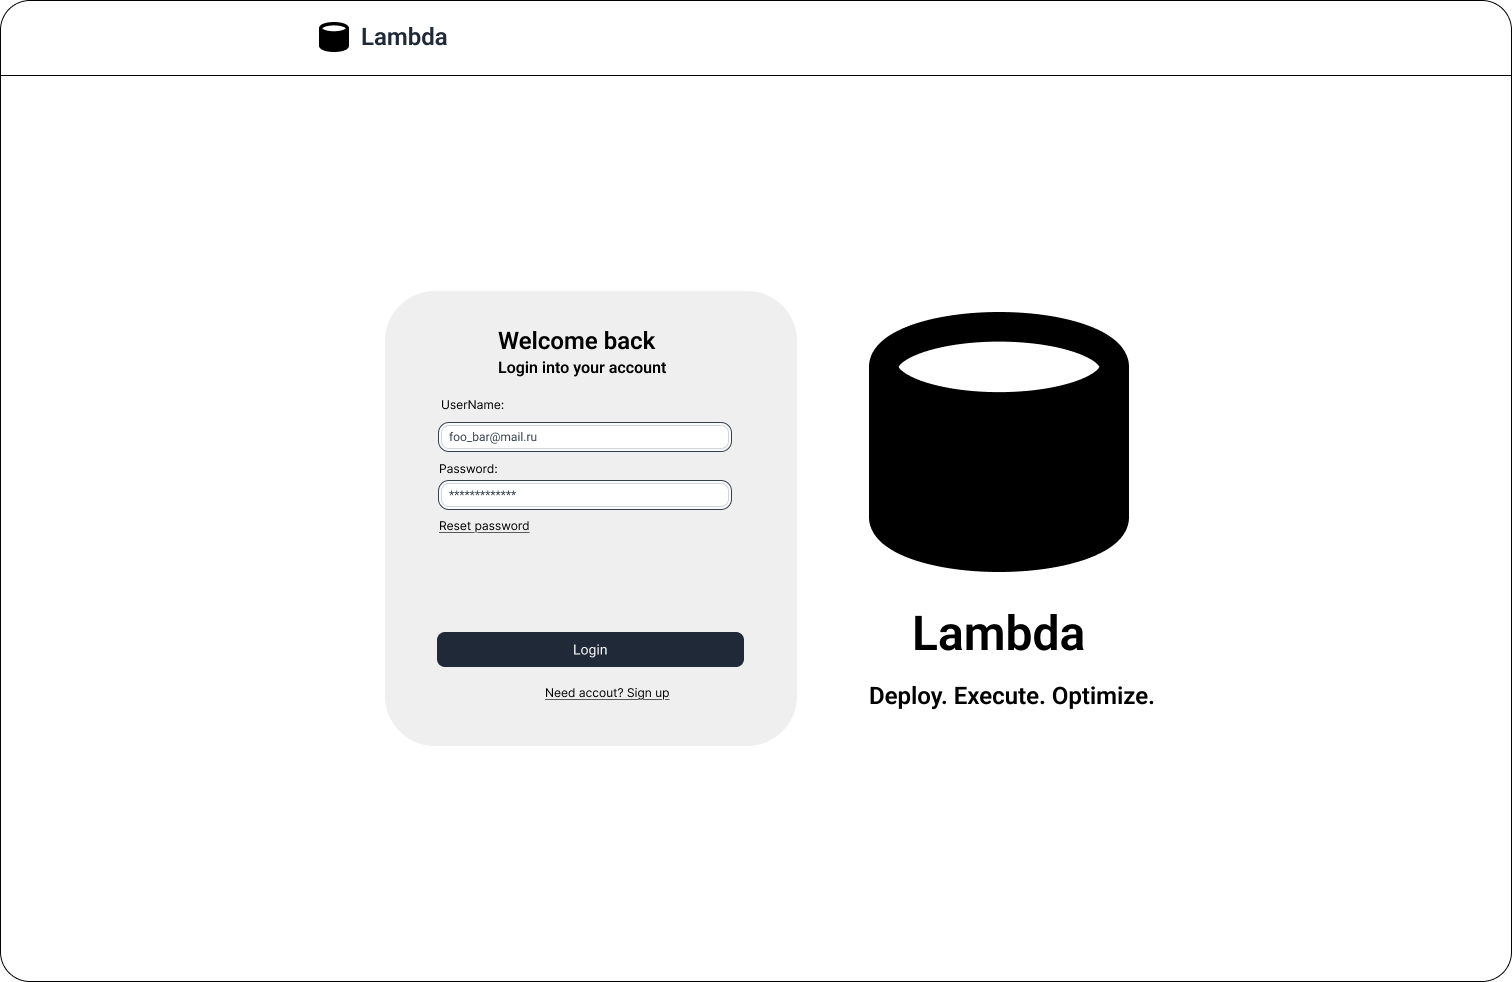
\includegraphics[width=\linewidth]{generated/Login-page.png}
  \caption{Каркасный макет страницы входа}
  \label{Login-page}
\end{figure*}

Для пользователей не имеющих учетной записи в системе, предстусмотре форма регистрации, которя доступная при переходе по ссылке, находящейся в нижней части формы входа. (Рис. ~\ref{Registration-page})

\begin{figure*}[!t]
  \centering
  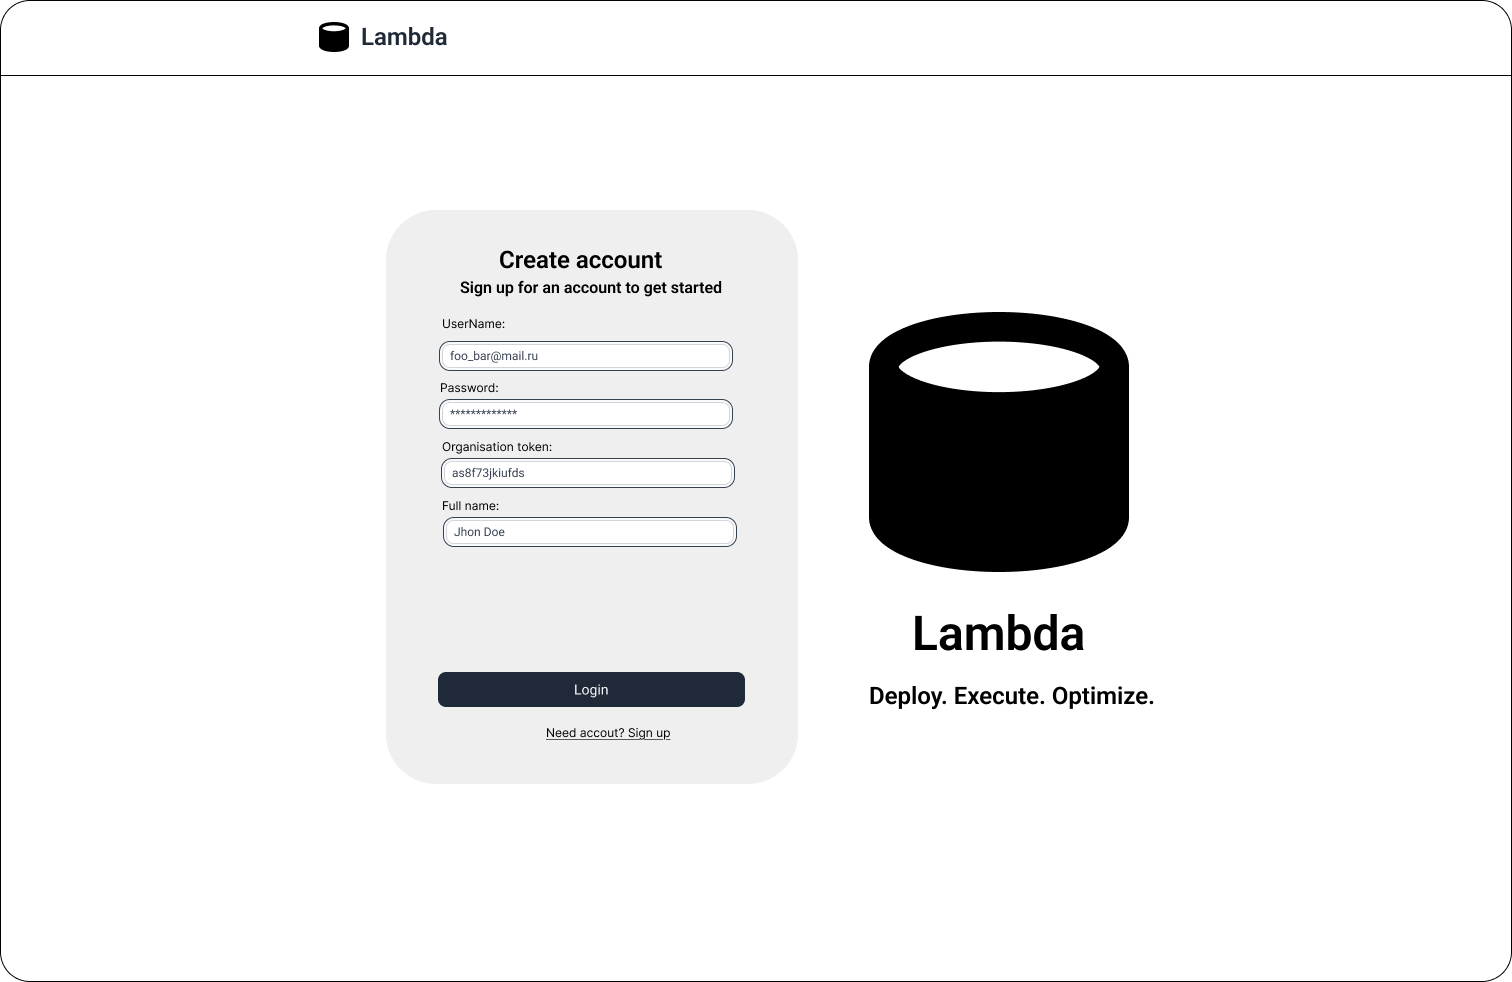
\includegraphics[width=\linewidth]{generated/Registration-page.png}
  \caption{Каркасный макет страницы регистрации пользователя}
  \label{Registration-page}
\end{figure*}

\subsection{Страница запущенных задач}

На странице запущенных задач располагается информация обо всех запущенных пользователем задачах (Рис. ~\ref{Jobs-dashboard}).

В верхней части страницы располагается счетчик всех, выполненных, запущенных задач и задач запущенных неудачно.
При нажатии накаждый из счетчиков применяется соответствующий фильтр к спску задач расположенному ниже.

При взаимодействии с каким либо из элементов задач, расположенных в списке задач, пользователь переходит на стриницу задачи.

\begin{figure*}[!t]
  \centering
  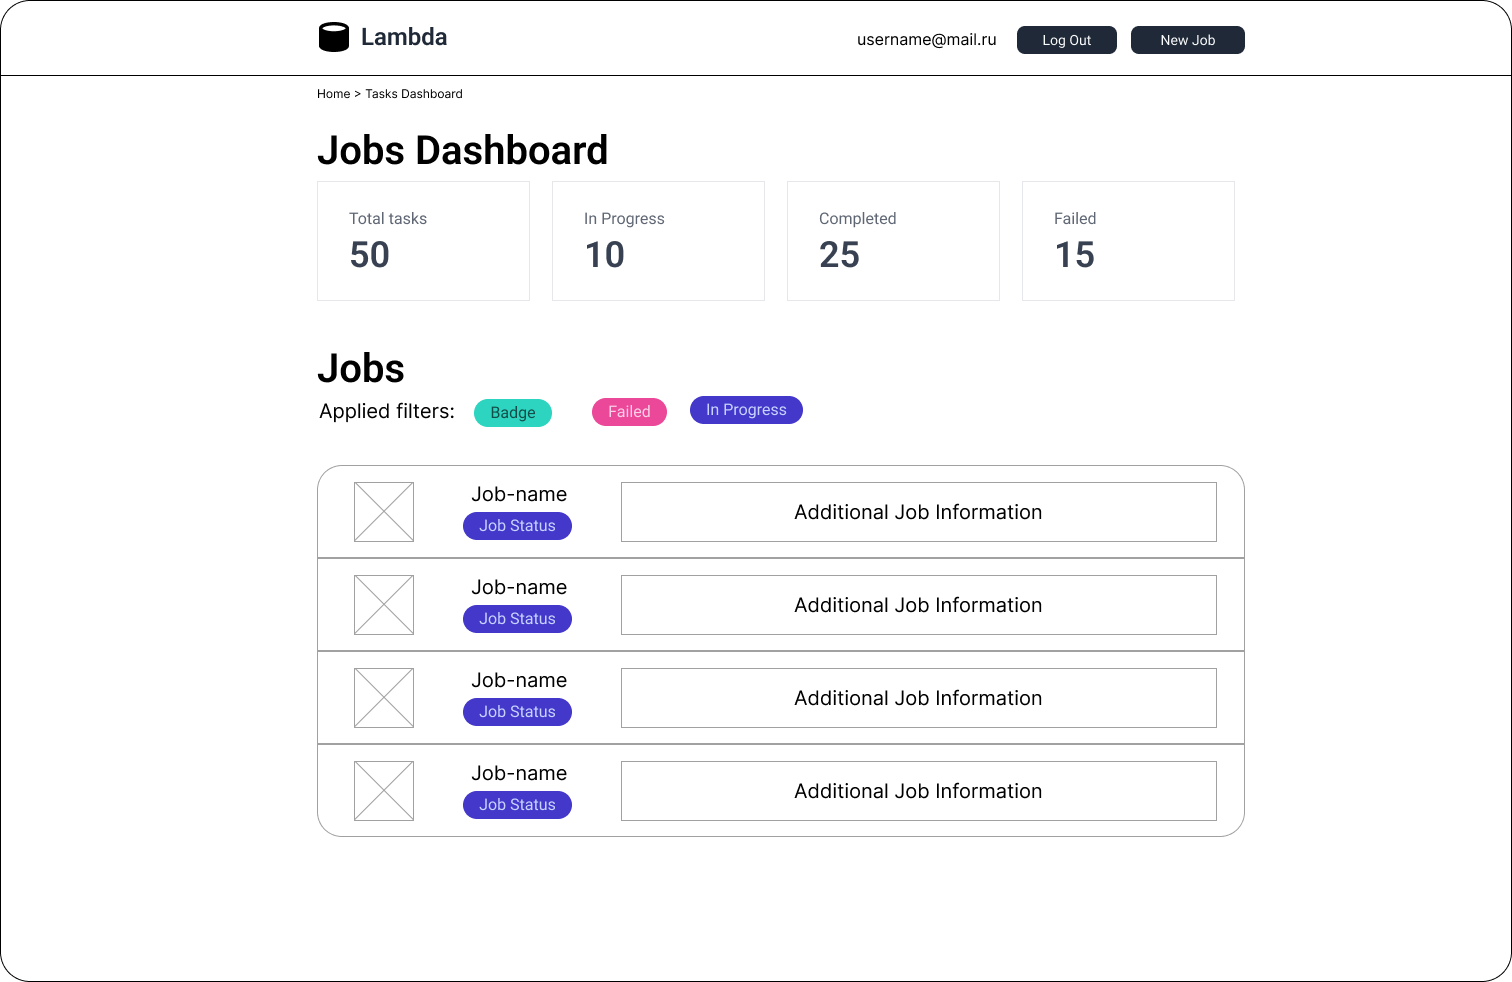
\includegraphics[width=\linewidth]{generated/Jobs-dashboard.png}
  \caption{Каркасный макет страницы запущенных задач}
  \label{Jobs-dashboard}
\end{figure*}

\subsection{Страница задачи}

На странице задачи располгается вся информация о задаче.

В Верхней части страницу расположены кнопки редактирования задачи, каоторая позволяет отредактировать параметры запуска задачи для будущих щапусков, и кнопка удаления задачи которая позволяет прекратить выполнение последующих запусков и скрыть от пользователей удаленную задачу.

В нижней части страницы располагается список запусков задачи. Если зажача запущена в данный момент отображается кнопка завершения выполнения. При взаимодействии с каким либо из элементов в списке запусков пользователь переходит на страницу запуска задачи.

\begin{figure*}[!t]
  \centering
  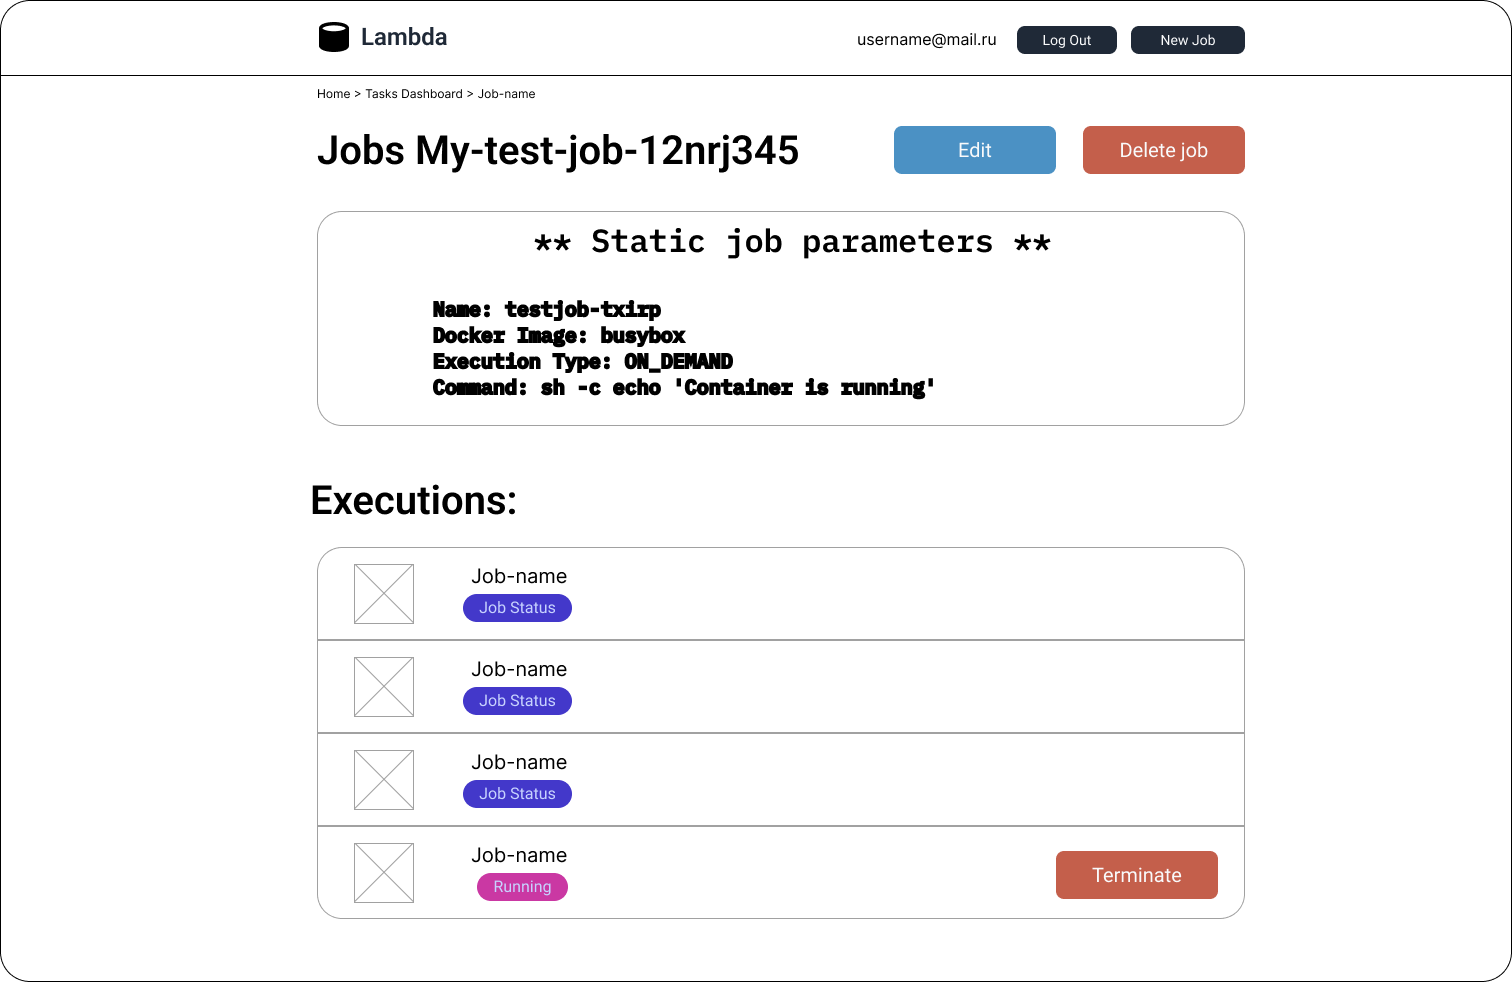
\includegraphics[width=\linewidth]{generated/Task-page.png}
  \caption{Каркасный макет страницы просмотра запущенной задачи}
  \label{Task-page}
\end{figure*}

На страницу запуска задачи отображается название задачи к которой относится запуск и порядковый номер запуска, кнопки выгрузки логов запуска, завершения выполнения запуска и логи выполнения. 

Окно просмотра логов продествляет собой зону просмотра текста с прокртку по осям X и Y.

\begin{figure*}[!t]
  \centering
  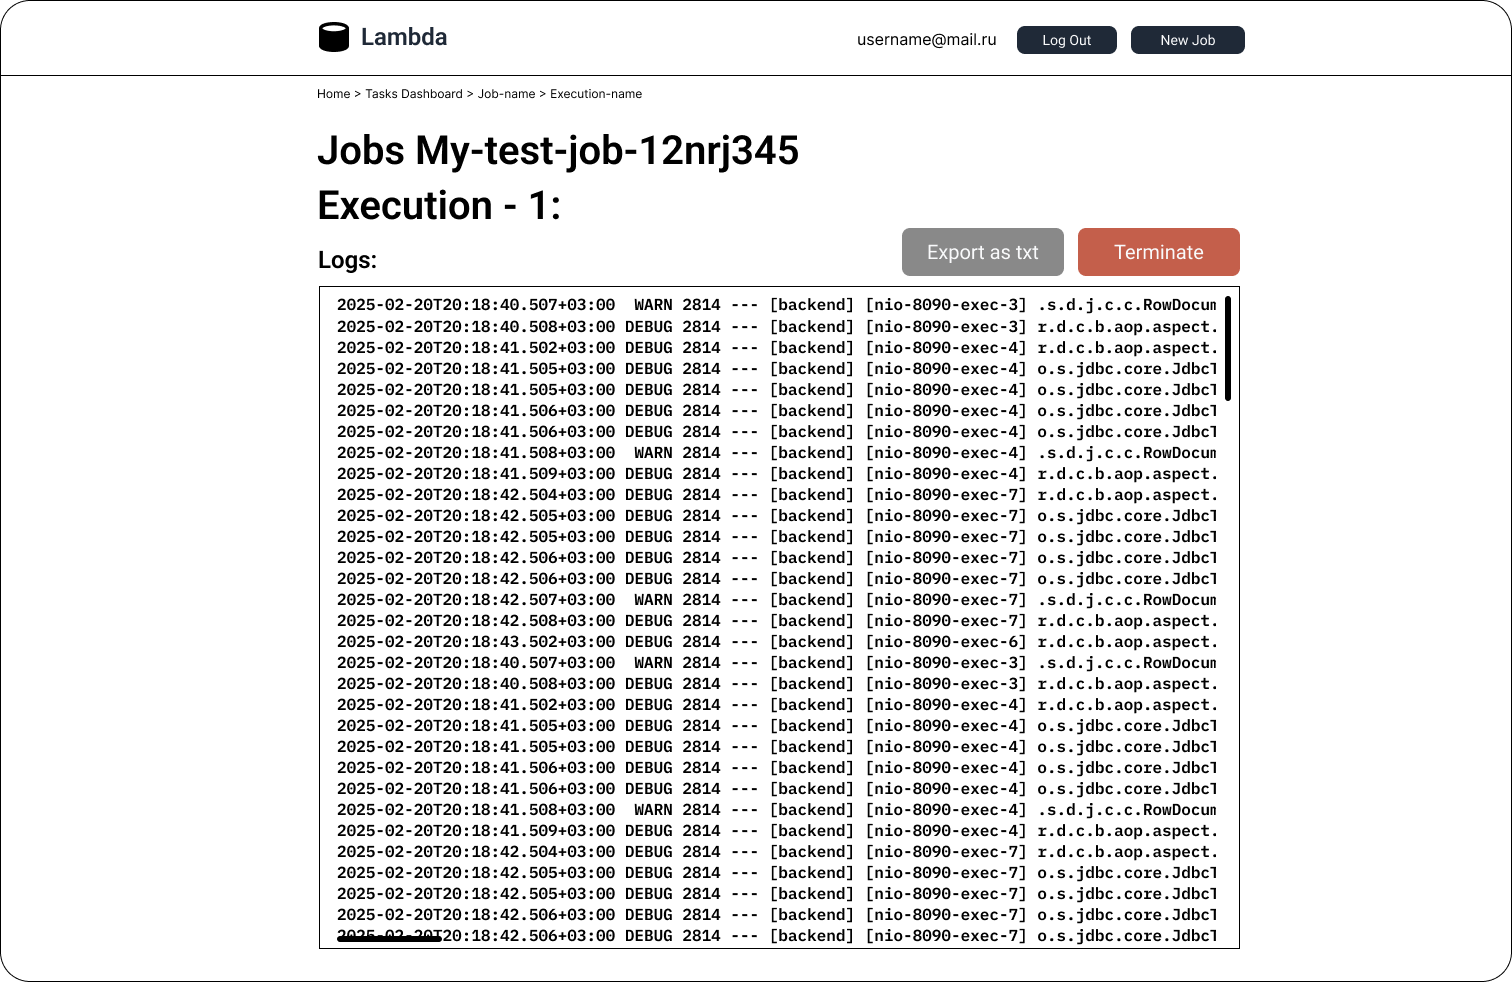
\includegraphics[width=\linewidth]{generated/Execution-page.png}
  \caption{Каркасный макет страницы просмотра запуска задачи}
  \label{Execution-page}
\end{figure*}

\subsection{Страница профиля пользователя}

На страницу профиля пользователя отображается информация о пользователе и о группах пользователей в которых он состоит.

Если пользователь состоит из какой либо группе ему отображется кнопка выхода из группы.

Если пользователь является членом группы администраторов, ему доступна форма генерации и копирования токена доступа в рабочее пространство группы.

В нижней части страницы отображается список участников группы.

Если пользователь является членом группы администраторов, ему доступно управление правами доступа дургих членов группы. Иначе чекбоксы находятся в неактивном состоянии.

\begin{figure*}[!t]
  \centering
  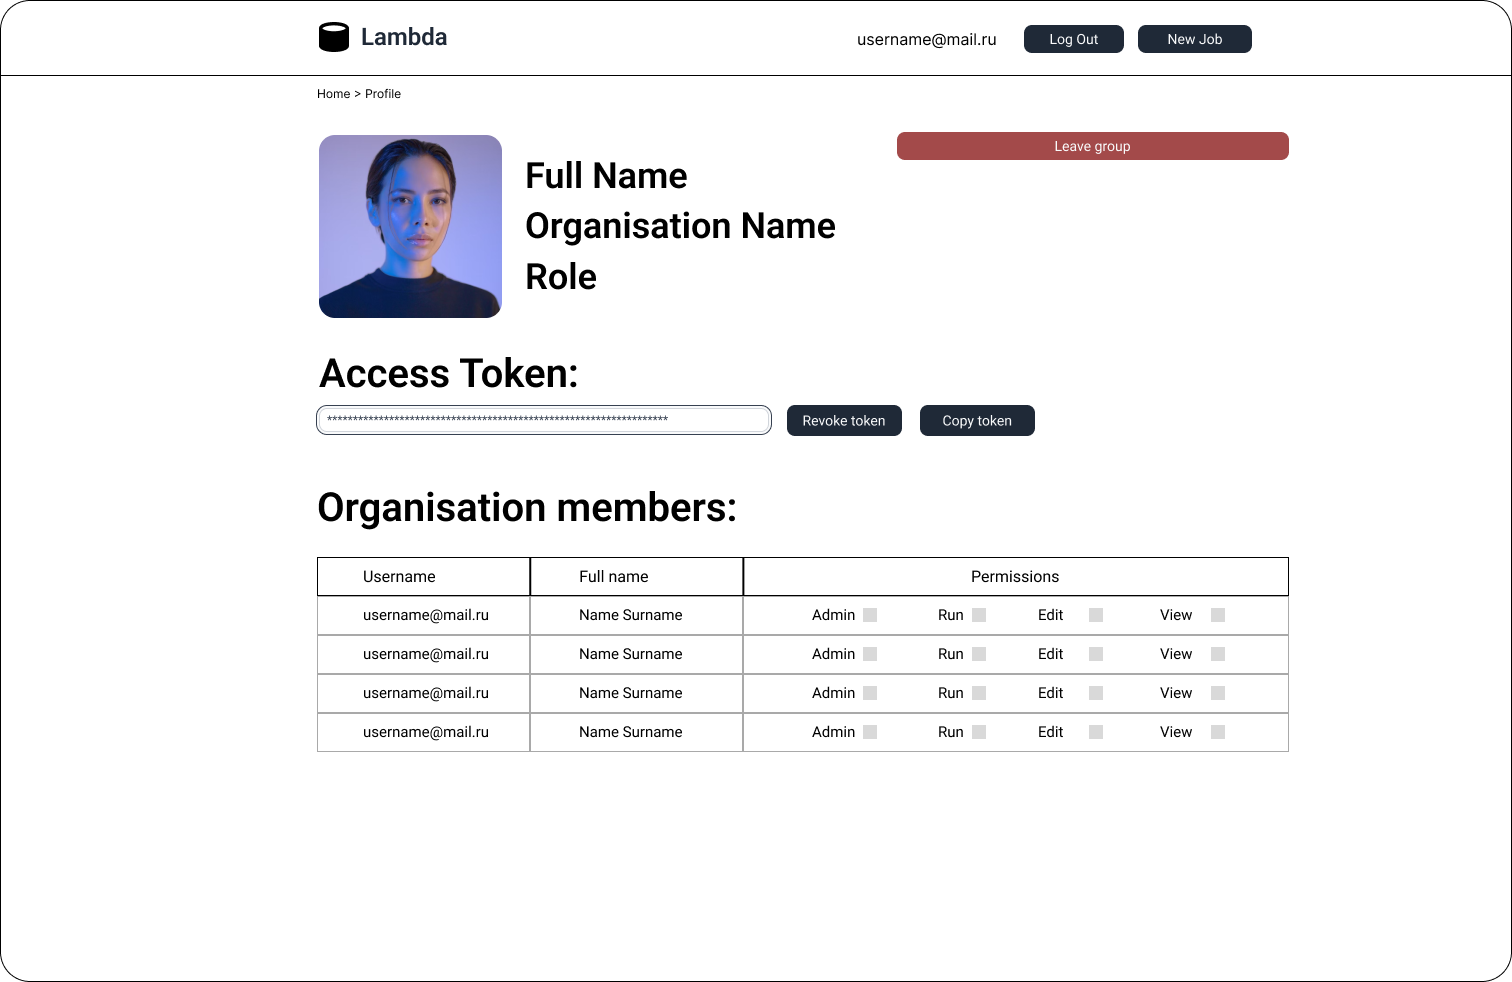
\includegraphics[width=\linewidth]{generated/Profile-page.png}
  \caption{Каркасный макет сраницы }
  \label{Profile-page}
\end{figure*}

\section{Разработка програмного интерфейса сервеной чаcти}

\subsection{Назначение и роль API в системе}

Прикладной прграммный интерфейс (API) \cite{ong2015materials} серверной части системы выступает ключевым элементом архитектуры, обеспечивая возаимодействие между киентами и сервисами разрабатываемой системы.

API в системе выполняет такие такие функции как:

\begin{itemize}
  \item[---] служит единой точной входят для всех клиентов;
  \item[---] предосталяет единый способ взаимодействия с системой.
\end{itemize}

Основными потребителями програмного интерфейса разрабатываемого серверного решение является веб-клиент платформы, а так же потребители webhook\cite{biehl2017webhooks} сервисов, предоставляемых платформой.

\subsection{Выбор архитектурного стиля прикладного программного интерфейса}

При проектировании серверной части критически важен выбор подхода и врхитектуры проектирования API.
Этот выбор определяет подходы взаимодействия между клиентом и сервером, а так же влияет на поизводительность, масштабируемость и простоту интеграции с разрабатываемым сервисом.
В настоящее время в проектировании API наиболее распространены 3 подхода: 

\begin{itemize}
  \item[---] REST\cite{wilde2011rest};
  \item[---] SOAP\cite{box2000simple};
  \item[---] Различные RPC протоколы\cite{srinivasan1995rpc}. 
\end{itemize}

В качестве архитектурного подхода к проектированию программного интерфейса выбран Representational State Transfer (REST).

Ключевыми аспектами в выборе REST как архитектурного подхода к проектированию программного инерфейса стали:

\begin{itemize}
  \item[---] широкое распространение и поддержка: rest является отраслевым стандартом при проектировании веб-API;
  \item[---] использование стандартных протоколов HTTP/HTTPS;
  \item[---] простота интеграции;
  \item[---] использоваение текстового кодирования данных: упрощает и ускоряет отладку. 
\end{itemize}

\subsection{Основные ресурсы и логические группы конечных точек}

Прикладной программный инерфейс платформы предусмотривает набор операций, позволяющих клиентам управлять ресурсами платформы.
К основыным ресурсам плфтормы можно онести:

\begin{itemize}
  \item[---] JwtToken - ресурс, представляющий набор данных, содержащих криптографические токены, необходимые для взаимодействия с конечными точками, защищенными механизмами авторизации;
  \item[---] User - ресурс, представляющий набор данных о пользователе, в том числе информацию о пользователе, о его ролях и группах в которых он состоит;
  \item[---] GroupDescription - ресурс, представляющий группу пользователей;
  \item[---] Permission - доступ к той или иной части функционала платформы в рамках группы пользователей и разделенных между ними ресурсами; 
  \item[---] Job - ресурс, представляющий информацию о задаче, включает все параметры выполнения задачи, а так же информацию о ее запусках;
  \item[---] ExecutionResult - ресурс, представляющий информацию о запуске задачи. 
\end{itemize}

Логически все конечные точки программного интерфейса системы можно разделить по различным наборам признаков: по доступности из неавторизованной зоны, по ресурсу, к которому конечная точка позволяет получить доступ, по наличию вляния на состояние системы.

Из неавторизованой зоны доступны только конечные точки, позволяющие польюзователю зарегистрироваться, пройти авторизацию или сбросить пароль.
К этой группе конечных точек относятся:

\begin{itemize}
  \item[---] POST /public/api/v1/authentication/reset-password;
  \item[---] POST /public/api/v1/authentication/log-in;
  \item[---] POST /public/api/v1/registration;
\end{itemize}

Все остальные конечные точки доступны только из авторизованой зоны.

По ресурсу, к которому контрольная точка предоставляет доступ конечные точки можно разделить на группы:

\begin{itemize}
  \item[---] Управление пользователями;
  \item[---] Управление групповым досутпом;
  \item[---] Управление запущенными задачами;
\end{itemize}

К группе конечных точек, позволяющих управлять пользователями относятся конечные точыеи доступные из неавторизованой зоны.

К группе конечных точек, позволяющих управлять групповым доступом польхователей относятся конечные точки:

\begin{itemize}
  \item[---] POST /api/v1/role-model/refresh-join-group-token/{groupId};
  \item[---] POST /api/v1/role-model/leave-group/{groupId};
  \item[---] POST /api/v1/role-model/join-group;
  \item[---] POST /api/v1/role-model/exclude-member-from-group;
  \item[---] POST /api/v1/role-model/create-group;
  \item[---] POST /api/v1/role-model/change-permission;
  \item[---] GET /api/v1/role-model/group/{groupId};
  \item[---] GET /api/v1/role-model/get-join-group-token/{groupId}.
\end{itemize}

К группе конечных точек, позволяюших управлять запущенными задачами относятся:

\begin{itemize}
  \item[---] GET /api/v1/job
  \item[---] POST /api/v1/job
  \item[---] POST /api/v1/job/webhook/run/{id}
  \item[---] POST /api/v1/job/rerun/{id}
  \item[---] POST /api/v1/job/delete/{id}
  \item[---] POST /api/v1/job/cancel/{id}
  \item[---] GET /api/v1/job/{id}
\end{itemize}

К группе конечных точек, позволяющих менять состояние ресурсов системы относятся все конечные точки использующие метод пост при выполнении http зпроса.

\subsection{Описание сценариев использования}

В системе предсумотрены различные сценарии использования API для выполнения задач управления удаленными вычислениями через плфторму.

К основным сценариям можно отнести:

\begin{itemize}
  \item[---] Авторизация пользователя;
  \item[---] Создание новой группы пользователей;
  \item[---] Добавление пользователя в группу;
  \item[---] Исключение пользователя из группы;
  \item[---] Добавление, отнимание доступов пользователя в рамках группы;
  \item[---] Просмотр списка участников группы и из доступов;
  \item[---] Получение списка запущенных задач и просмотр результатов выполнения;
  \item[---] Создвние новой задачи;
  \item[---] Перезапуск, остановка, удаление задачи.
\end{itemize}

{\bf Авторизация пользователя }

Пользователь может пройти авторизацию вызвав конечную точку POST /public/api/v1/authentication/log-in.

Если пользователь не имеет учетной записи в системе он может ее создать вызвав конечную точку POST /public/api/v1/registration.

Ответом сервера при входе и регистрации будет пара Jwt токенов\cite{ahmed2019authentication}, которые пользователь должен использовать для доступа к конечным точкам защещиенным механизмами авторизации.

Если пользователь уже имеет учетную запись, но забыл от нее пароль, он может его сбросить, при вызове эндпоинта reset-password.

{\bf Сценарии управления группами пользователей }

Групповая модель доступа к ресурсам разрабатываемой системы предполагает гибкую систему групп и доступов, позволяющую разграничивать доступ к ресурсам платформы у различных пользоватлей.

По умолчанию пользователь не состоит ни в какой группе и может создавать и просматривать задачи только от своего имени.

Для того что бы создать группу пользователей необходимо вызвать конечную точку POST /api/v1/role-model/create-group. Пользователь, создавший группу, будет назначен ее администратором, а так же ему будут присвоены все дуступы в рамках созданной группы.

Для того что бы добавиьт пользователя в группу предусмотрен механизм токенов доступа в группу.
Администратор группы может запросиьт токен доступа вызвав конечную точку GET /api/v1/role-model/get-join-group-token.
Дальше токен любым удобным способ отправляется пользователю который должен вступить в группу.

Что бы присоединиться к группе необходимо вызвать конечную точку POST /api/v1/role-model/join-group.
Пользователь будет добвален в группу с доступом на просмотр по умолчанию.
Для того что бы расширить перечень доступов пользователя в рамках группы, администратор группы должен произвети соответсвующие операции.

Для добаления или удаления доступа у пользователя, являющегося членом группы, администратор должен воспользоваться конечной точкой POST /api/v1/role-model/change-permission.

Пользователь может покинуть группу используя конечную точку POST /api/v1/role-model/leave-group/\{groupId\}.

Администратор так же может исключить пользователя из группы используя конечную точку POST /api/v1/role-model/exclude-member-from-group.

{\bf Просмотр, создание и управление запущенными задачами }

Пользователь может создать задачу доступную только ему или членам группы по его выбору вызвав эндпоинт POST /api/v1/job.

Запросить список текущих задач можно вызвав эндпоинт GET /api/v1/job.

В зависимости от членства в различных группах и наличия соответствующих доступов у пользователя, при запросе текущих задач он получит список задач доступных ему или члеам группы в которую он входит и имеет доступ на просмотр.

Отдельную задачу можно получить вызвав эндпоинт GET /api/v1/job/{id}.

При наличии досупа пользовать может перезапустить задачи при помощи эндпоинта POST /api/v1/job/rerun/{id}, отменить выполнение задачи POST /api/v1/job/cancel/{id} или удалить задачу POST /api/v1/job/delete/{id}.

Если задача является веб-хуком, то пользватель может его вызвать через интерфейс или API плфтформы возмользовавшись конечной точкой POST /api/v1/job/webhook/run/{id}.

\section{Разработка сервеной части}

\subsection{Архитектура серверной части}

Серверная часть система является распределенным приложеним, в котором монолитное веб приложение служит связующим компонентом между другими частями системы.
Основу системы соствляет веб-приложение, написанное на языке Kotlin и фреймворке для написания веб-приложений Spring Boot.

Помимо разрабатываемого приложения ключевыми компонентами системы являются кластер Kubernetes, в котором разворачиваются сервисы платформы и пользовательские задачи, база данных PostgreSQL, выполняющая функции хранения данных веб-прложения и сервера авторизации, а так же сервер авторизации Keycloak, выполнязий задачи упроавления токенами доступа пользователей и хранения информации о ролях и доступах пользователей.

\subsection{Реализация REST API}

REST API платформы спроетирован в соответсвие с подходами ресурс-ориентированной архитектуры(ROA)\cite{guinard2011internet} и использует стандарт OpenAPI 3.0 для описания конечных точек.

Конечные точки платформы сгруппированы по функциональным областям - регистрация и авторизация, управление групповым доступом, управление жизненным циклом задач.

Версионирование приклодного инфтерфейса плфтформы осуществляется путем досбавления префикса v1 перед названием группы конечных точек, таким образом при дальнейшем развитии платформы, при отсутствии обратной совместимоти могут безопасно эволюционировать.

Система авторизации разрабатываемой системы использует протокол OAuth 2.0\cite{boyd2012getting} для авторизации пользователей.
За генерацию и валидацию JWT-токенов\cite{ahmed2019authentication} отвечает сервер авторизации Keycloak.

Механизмы авторизации, основанные на использовании JSON Web Token передают данные о пользователе в незашифрованном виде.

Каждый JWT токен состит из трех частей:

\begin{itemize}
  \item[---] заголовок - содержит название алгоритма подписи токена;
  \item[---] полезная нагрузка(payload) - набор утверждений(claims) о пользователе;
  \item[---] подпись токена - HMAC-хэш, вычисленный сервром авторизации с использованием приватного ключа.
\end{itemize}

Полезная так как JWT-токен передает полезную нагрузку в незашифрованном виде, утверждения о пользователе не должны содержать какой либо чувствительной информации.
Подмена утверждений содержащихся в токене невозможна так как при изменении набора утверждений, неизбежно изменится их хеш, содержащийся в последней части токена и вычисляемый с использованием приватного ключа, который известен только серверу авторизации. Таким образом гарантируется безопасность доступа к ресурсом платформы.

В листинге \ref{lst:acces_token} предаствлен пример расшифрованного токена доступа, которым оперирует платформа.

\begin{lstlisting}[caption={Токен доступа}, label=lst:acces_token]
  {
    "exp": 1743891730,
    "iat": 1743855730,
    "jti": "59864e52-01f6-4781-a342-6e32f444eb90",
    "iss": "http://localhost:8080/realms/users",
    "aud": "account",
    "sub": "84e487cc-a864-462c-8074-bbb4d020c380",
    "typ": "Bearer",
    "azp": "backend-client",
    "sid": "9dd6e8b2-54d8-45e5-a325-2874b4090c81",
    "acr": "1",
    "allowed-origins": [
      "/*"
    ],
    "realm_access": {
      "roles": [
        "default-roles-users",
        ...
        "offline_access"
      ]
    },
    "resource_access": {
      "account": {
        "roles": [
          "manage-account",
          "manage-account-links",
          "view-profile"
        ]
      }
    },
    "scope": "profile email",
    "email_verified": true,
    "preferred_username": "a@mail.ru"
  }
\end{lstlisting}

При проектировании авторизации платформы, критическим требованием была реализация платформы без редиректов, из-за этого было принято решение отказаться от использования форм авторизации Keycloak и реализовать собственный API авторизации, делегировав серверу авторизации лишь задачи генерации и валидации токенов.

\subsection{Технологии и архитектура веб-сервиса}

Спроектированный веб-сервис реализует построен с ипользованием распространенного паттерная шестигранной архитектуры\cite{richardson2023microservices} и соблюдает приципы второго уронвня модели зрелости Ричардсона\cite{salvadori2015maturity}. 

На уровне приложения находятся сервисы платформы, отвечающие за реализацию бизнес логики работы с доменными сущностями. К таким сервисам относятся:

\begin{itemize}
\item[---] AuthenticationService;
\item[---] ExecutionService;
\item[---] JobService;
\item[---] RegisterUserService;
\item[---] UserService.
\end{itemize}

В этих сервисаз содержится бизнес-логика отвечающая за согласнованную работу системы и выполнение ей, возложенных на нее задач.

С Application слоем взаимодейтвует слой контроллеров, к оторому относятся следующие классы:

\begin{itemize}
\item[---] AuthenticationController;
\item[---] JobController;
\item[---] RegistrationController;
\item[---] RoleModelController;
\item[---] UsersController.
\end{itemize}

Слой контроллеров отвечает за обработку входящих запросов и преобразование ответов сервисного слоя в сущности ResponseEntity.

Маршрутизацией трафика на конечные точки, объявленные в контроллерах занимается веб-сервер Tomcat.

Для звамодействия с базой данных спользуется слой DAO (Data Acess Object). 

Для работы с информацией, хранящейся в базе данных исопльзуется порход ORM (Object Relational Mapping)\cite{o2008object}. Данный подход реализован с испльзованием стандарта JPA (Java Persitance API)\cite{yang2010java}, который реализуется библиоткеой Spring Data JDBC, предоставляющей лаконичный API для взаимодействия с базой данных, а так же легко интеграруемой с основным фреймворком приложения Spring Boot.

На слое DAO представлены два типа сущностей - Entity и Repository.

Entity классы предствляют собой отражение доменных сущностей хранящихся в базе данных, к ним относятся пользователи, задачи и результаты выполнения задач. 

Repository в свою очередь является классом, позволяющим получить и менять состояние Entity которой он управляет. На слое DAO представлены следующие репозитории:

\begin{itemize}
\item[---] ExecutionResultRepository;
\item[---] GroupAccessTokenRepository;
\item[---] JobRepository;
\item[---] UserRepository.
\end{itemize}

На интеграционнном слое приложения располагаются сервисы, обеспечивающие взаимодействие с другими сервисами платформы. К таким сервисам относятся KeycloakService, реализующий интеграцию с сервером авторизации Keycloak и KubernetesService, позволяющий взаимодейстоввать с кластером Kubernetes, в котром разворачиваются создаваемые пользователями задачи.

Для взаимодействия с Keycloak адаптер KeycloakService использует клиентскую библиотеку $org.keycloak:keycloak-admin-client$, котороя является тонким клиентом для сервера авторизации кейлок, предоставляя удобный DSL (Domain Specific Language)\cite{mernik2005and} интерфейс для взаимодействия с сервром авторизации. Библиотека берет на себя функции управления токенами досутпа, кешированными локально на стороне клиента, а так же за преобразование сущностей DSL в вызовы REST API сервера авторизации.

Адаптер KubernetesService использует библиотеку $io.kubernetes:client-java$ для взаимодействия с подчиненным кластером Kubernetes. Подключение к кластеру устанавливается при помощи файла конфигурации $.kubeconfig$, путь к которому задан в переменной окружения $\$KUBECONFIG$.

Клиентаская библиотка так же является тонким клиентом для Kubernetes и предоставляет удобный DSL API для генерации манифестов Kubernetes\cite{poulton2023kubernetes}, а так же предоставляет удобные абстракции для вызова метдов $Kubernetes$ $API Server$.

\subsection{Интеграция с Kubernetes}

Для обеспечения изоляции пользовательских задач от сервисов платформы, реализован подрход разделения пространств имен.
Исопльзуются два основыных пространства:

\begin{itemize}
\item[---] пространство $default$ - служит для развертывания системных сервисов, таких как разработнный веб-сервис, север авторизации, база данных.
\item[---] пространство $sandbox$ - предназначено для развертывания пользовательских задач. 
\end{itemize}

Такое разделение позволяет минимизировать риск несанкционированного досутпа к ресурсам платформы и предотвратить риск возможных конфликтов именования ресурсов платформы.

Для реализации возможности создания пользователь задач используеются встроенные сущности Kubernetes Job и CronJob.
KubernetesService управлет жизненным циклом объектов выполняя следущие операции:

\begin{itemize}
\item[---] создание ресурсов;
\item[---] получение статуса выполнения;
\item[---] получение логов выполнения;
\item[---] остановка и удаление.
\end{itemize}

За генерацию манифестов отвечает фабрика\cite{cooper2000java} $V1JobFactory$. 
В этом классе инкапсулирована логика преобразования параметро создания задачи $JobParameters$ в манифест Kubernetes.

Ключевые аспекты конфигурации включают:

\begin{itemize}
\item[---] установку $metadata.name$ для идентификации $Job$ и $CronJob$;
\item[---] определение спецификации контейнера ($V1Container$), включая образ ($image$), команду ($command$) и переменные окружения ($env$);
\item[---] установку политики перезапуска $restartPolicy$ в значение $Never$ для $Pod$, создаваемых в рамках $Job$, что соответствует семантике выполнения задачи до завершения;
\item[---] конфигурацию $backoffLimit$ для $JobSpec$, определяющую количество попыток перезапуска в случае сбоя;
\item[---] для $CronJob$ дополнительно указывается поле $schedule$ и шаблон $jobTemplate$.
\end{itemize}

После запуска задачи сервис $ExecutionService$ периодически опрашивает $KubernetesService$ для актаулизации статуса выполнения задачи.
Собранная аггрегированная информация о статусе выполнения задачи исопльзуется для обновления информации о задаче в базе данных, откуда в последствии данная информация будет доставлена пользователям.

\subsection{Интеграция с Keycloak и реализация механизмов ролевого доступа}

Основное взаимодействие разработанного веб-сервиса с сервером авторизации Keycloak сокрыто в классе $KeycloakService$.
Вся информация об учетной записи пользователя хранится на сервере авторизации.
$KeycloakService$ API предосталяет достаточный функционал для управления жизненным циклом учетной записи пользователя.

Изнетграция с Keycloak осуществляется через экземляр DSL-фабрики Keycloak.
В процессе формирования обращений к API Keycloak ключевыми сущносятми, в которые преобразуются доменные сущности платформы, являются:

\begin{itemize}
  \item[---] UserRepresentation - DTO (Data Transfer Object) пользователя Keycloak;
  \item[---] CredentialRepresentation - DTO учетных данных пользователя;
  \item[---] GroupRepresentation - DTO группы пользоватей Keycloak;
  \item[---] RoleRepresentation - DTO роли уронвя realm Keycloak.
\end{itemize}

Для поддержания фукционалности управления ролевым доступом реализованы межанизмы генерации ролей уровня realm на основании идентификатора группы и доступа который присваиватся опльзователю в рамках этой группы.

В рамках модели группа --- доступ, роли, присваиваемые пользователю именуются по шаблону:
$$
\{Permission\_Name\}/\{Group\_UUID\}
$$

Такой подход к организации доступов пользователя позволят выдать пользователю разный набор досутпов в разных группах, исключая возможность пересечения досутпов между группами.

В последстии в токене доступа, в утверждении $realm\_access.roles$ созданные роли принимают вид представленный в листиге \ref{lst:roles_in_token}.

\begin{lstlisting}[caption={Пример представления ролей пользователе в токене досутпа}, label=lst:roles_in_token]
...
    "realm_access": {
      "roles": [
        "RUN/1b1d286b-1a33-4c17-8dda-d9a1b4037253",
        "ADMIN/1b1d286b-1a33-4c17-8dda-d9a1b4037253",
        "EDIT/216ef3cf-aa7c-4612-85f0-fad77f3a3637",
        "VIEW/1b1d286b-1a33-4c17-8dda-d9a1b4037253",
        "EDIT/1b1d286b-1a33-4c17-8dda-d9a1b4037253"
      ]
    },
...
\end{lstlisting}

\subsection{Обработка авторизации пользователя}

Контроль за доступом к ресурсам плфотрмы яфляется критически важным спктом разработки системы. В системе реализованы механизмы валидации токенов доступа пользователей, а так же механизмы раздедедения конечных точек на авторизованную и неавторизовванную зоны.

\subsubsection{Интеграция с Keycloak и конфигурация Spring Security}

Интеграция с сервером авторизации Keycloak, для валидации токенов досутпа пользователей, осуществляется с использованием стандартных механизмов Spring Boot для конфигурации OAuth 2.0 Resource Server\cite{ferry2015security}.

Пример конфигурации ресурсного сервера представлен в листинге \ref{lst:resource_server_config}.

\begin{lstlisting}[caption={Конфигурация Resource Server}, label=lst:resource_server_config]
...
  spring:
    security:
      oauth2:
        resourceserver:
          jwt:
            issuer-uri: http://keycloak:8080/realms/users
...
\end{lstlisting}

Ключевым аспектом конфигурации является указание парметра $issuer-uri$, определяюзего адрес сервера, выпустившего JWT-токены досутпа, которым доверяет веб-сервис.

При образении на конечную точку $issuer-uri$, Keycalok предоставляет набор публичных ключей, с помощью которых веб-сервис может валидировать токен досутпа в запросе. Пример ответа сервера авторизации на запрос публичных ключей представлен в листиге \ref{lst:iss_uri_response}.

\begin{lstlisting}[caption={Ответ на запрос публичного ключа}, label=lst:iss_uri_response]
...
{
  "realm": "users",
  "public_key": "MIIBIj...QAB",
  "token-service": "http://keycloak:8080/realms/users/protocol/openid-connect",
  "account-service": "http://keycloak:8080/realms/users/account",
  "tokens-not-before": 0
}
...
\end{lstlisting}

При получении ответа сервера авторизации с публичным ключем, Security middleware проверят токен досутпа по следующим параметрам:

\begin{itemize}
\item[---] Подпись токена: Проверяется с использованием публичного ключа, полученного от Keycloak по $issuer-uri$.
\item[---] Срок действия (Expiration): Проверяется, не истек ли срок жизни токена ($exp$ утверждение).
\item[---] Издатель (Issuer): Проверяется соответствие значения iss claim в токене сконфигурированному $issuer-uri$.
\end{itemize}

\subsubsection{Конфигурация правил доступа в Spring Security}

Для разграницения досутпа у конечным точкам, требуюзим авторизованный доступ, исопзьуется бибилитека Spring Security.
Класс $SecurityConfig$ является единым местом настройки политик доступа к сервисам платформы.

Для сервисов платформы применяются следующие политики досутпа:

\begin{itemize}
  \item[---]Пути, начинающиеся с /public/**, пути для Swagger UI (/v3/api-docs/**), доступны всем пользователям без аутентификации.
  \item[---]HTTP-метод OPTIONS разрешен для всех путей для корректной работы механизма Cross-Origin Resource Sharing (CORS)\cite{arai2024method}, который используется при взаимодействии frontend-приложения с backend API из разных источников (доменов).
  \item[---]Все остальные запросы требуют наличия валидного JWT-токена в заголовке Authorization: Bearer <token> (authenticated()).
  \item[---]Отключение CSRF\cite{barth2008robust}: Защита от Cross-Site Request Forgery отключается, так как JWT-аутентификация является stateless и не подвержена данному типу атак в той же мере, что и сессионная аутентификация.
  \item[---]Настройка обработки JWT: Секция $oauth2ResourceServer().jwt()$ конфигурирует Spring Security для работы в режиме ресурсного сервера, ожидающего JWT-токены. Здесь же подключается пробразователь токенов KeycloakJwtTokenConverter, преобразущий утверждения токена доступа в Principal объект Spting Secutiry.
\end{itemize}

\subsubsection{Извлечение данных пользователя и ролей из JWT}

После успешной валидации токена Spring Security создает вспомогательный объект Authentication и помещает его в SecurityContextHolder, который доступен глобально в любом месте выполнения запроса.

Для удобного доступа к данным пользователя и его ролям, извлеченным из токена, используется абстракция getUserAuthentication над хранилищем SecurityContextHolder, позволяющая пребразовать его в удобный вспомогательный DTO класс UserAuthentication, хранящий информацию об идентификаторе и ролях пользователя.

\subsection{Обработка ошибок и логгирование}

В рамках платформы реализован функционал глобального логгирования вызовов метдов и обработки ошибок. 
Современные подходы к разработке для решение задач реализации сквозного фнукцилонала, затрагивающего большое колличество различных мест программы, но при этом реализующего схожий функционал предлагают внедрения AOP(Aspect Oriented Programming)\cite{kiczales1997aspect} для решения такого рода задач. 

\subsubsection{Централизованная обработка ошибок REST API}

Реализация единой обработки ошибок выполнена с использованием класса ErrorHandler. Аннотация @ControllerAdvice в Spring Boot позволяет классу перехватывать исключения, выброшенные из любого контроллера в приложении.

Класс ErrorHandler перехватывает все исключения возникающие в системе и производит над ними следующие действия:

\begin{itemize}
  \item[---]В лог записывается информация об ошибке, включая HTTP-метод, URI запроса, тип исключения и его сообщение.
  \item[---]Создается объект RestError, содержащий стандартизированную структуру данных об ошибке: HTTP-статус, общее сообщение об ошибке и детальное сообщение.
  \item[---]Сформированный RestError оборачивается в класс ResponseEntity с соответствующим HTTP-статусом. Это гарантирует, что клиент всегда получит ответ в предсказуемом JSON-формате, даже в случае непредвиденных сбоев на сервере.
\end{itemize}

Такой подход упрощает разработку клиентской части так как логика обработки ошибок стандартизирована.

\subsubsection{Логирование выполнения методов с использованием АОП}

Логирование является ключевым инструментом для отладки, мониторинга и анализа поведения системы.
Однако, внедрение логирующих вызовов непосредственно в бизнес-логику методов может приводить к зашумлению кода и нарушению принципа единственной ответственности.
Для решения этой проблемы реализован логгирующий аспект RestLoggingAspect.

Преимуществом данного подхода является декларативность. Достаточно пометить требующий логирования метод аннотацией @LogExecution, и аспект автоматически добавит необходимую логирующую обвязку без модификации исходного кода самого метода. Это значительно повышает читаемость и поддерживаемость кода бизнес-логики.

\section{Разработка клиентской части}

Для платформы развертывания контейнеризиованных функций разработано клиентское веб-приложение.
Оно позволяет обеспечить возаимодействие пользователя с автоматизированной системой.

Основной целью разработки разработки клиентского приложение является создание интуитивного, простого и понятного пользовательского интегрфейса (UI), позволяющего в полной  мере использовать доступный функционал платформы.

\subsection{Выбор стека технологий и инструментов}

Для разработки пользовательского интерфейса выбран фреймворк Vue3. К плюсан выбранного фреймворка можно отнести поддержку реактиваности в интерфейсе, богатую экоситему библиотек, производительность и размер бандла скомпиллированного приложения.

Для управления состояниями клиентского приложения выбран стэйт-менеджер Pinia.

Pinia для фреймворка Vue3 поставлется как стейт-менеджер по умолчанию, что обеспечиват легкую интеграцию библиотеки с фреймворком, в то же время является самой удобной и гибкой реализаций менеджера состояний приложения среди аналогов.

К основным преимуществам Pinia можно отнести:

\begin{itemize}
\item[---]официальная рекомендация для Vue 3;
\item[---]простота API, модульность;
\item[---]интеграция с Vue DevTools;
\item[---]поддержка TypeScript.
\end{itemize}

Для управления стилизацией HTML-элементов выбрана комбинация библиотек TailwindCSS и DaisyUI.

TailwindCSS реализует подход "utility-first". Вместо предопределенных классов компонентов, он предоставляет обширный набор низкоуровневых служебных классов, каждый из которых отвечает за одно конкретное CSS-свойство. Это позволяет разработчикам создавать полностью кастомные дизайны непосредственно в HTML-разметке, не покидая контекст и не создавая большие объемы пользовательского CSS. Такой подход обеспечивает максимальную гибкость в стилизации элементов интерфейса в точном соответствии с требованиями дизайна. Использование TailwindCSS позволять уменьшить использование CSS в проекте а так же ускорят разработку.

DaisyUI функционирует как плагин для TailwindCSS, предоставляя набор готовых, стилизованных компонентов пользовательского интерфейса (кнопки, формы, карточки, модальные окна, оповещения и т.д.). Важно отметить, что эти компоненты построены с использованием утилит TailwindCSS. Это позволяет значительно ускорить разработку стандартных элементов UI, так как не требуется собирать их с нуля из отдельных утилит.

Использвоание DaisyUI дайет неоспоримое преимущество - консистентность дизайна интерфейса прижения, достигается минимальными усилиями разработчика. Таким образом выбор DaisyUI многократно ускоряет прототипирование и делает результат намного более качественным.

\subsection{Архитектура клиентского приложения}

Структурно компоненты клиентского приложения разделены на несколько групп, объединенных общей функциональностью.

К основным группам компонентов можно отнести следующие:

\begin{itemize}
  \item[---] View - компоненты отвечающие за отображение страниц приложения;
  \item[---] Component - компоненты интерфейса, располагающиеся на страницах приложения;
  \item[---] Api - сервисы, позволяющие взаимодействовать с серверной частью приложения;
  \item[---] Store - модули ханилища состояния приложения, позволяющие различным компонентам приложения обмениваться информацией.
  \item[---] Utils - утилитарные компоненты, позволяющие решать специфические задачи, такие как управление и настройка сетевых соединений, работа с сессиоными хранилищами, управление поллингом запросов и маршрутизацией. 
\end{itemize}

\subsection{Реализация ключевых пользовательских сценариев и компонентов}

Клиентское приложение построено на основе компонентной архитектуры Vue.js, где каждый пользовательский сценарий реализуется через взаимодействие одного или нескольких компонентов, хранилищ состояния (Pinia) и сервисов для работы с API. Ниже рассмотрены основные сценарии и их реализация.

\subsubsection{Аутентификация и Регистрация}

Аутентификация и регистрация обеспечивают безопасный доступ пользователей к функциям платформы. В клиентской части эти процессы реализуются через набор компонентов представление LoginView содержит формы LoginForm, RegisterForm, ResetPasswordForm для ввода и валидации учетных данных. Компонент AuthSwitch реализует навигацию между входом и регистрацией.

\begin{figure*}[!t]
  \centering
  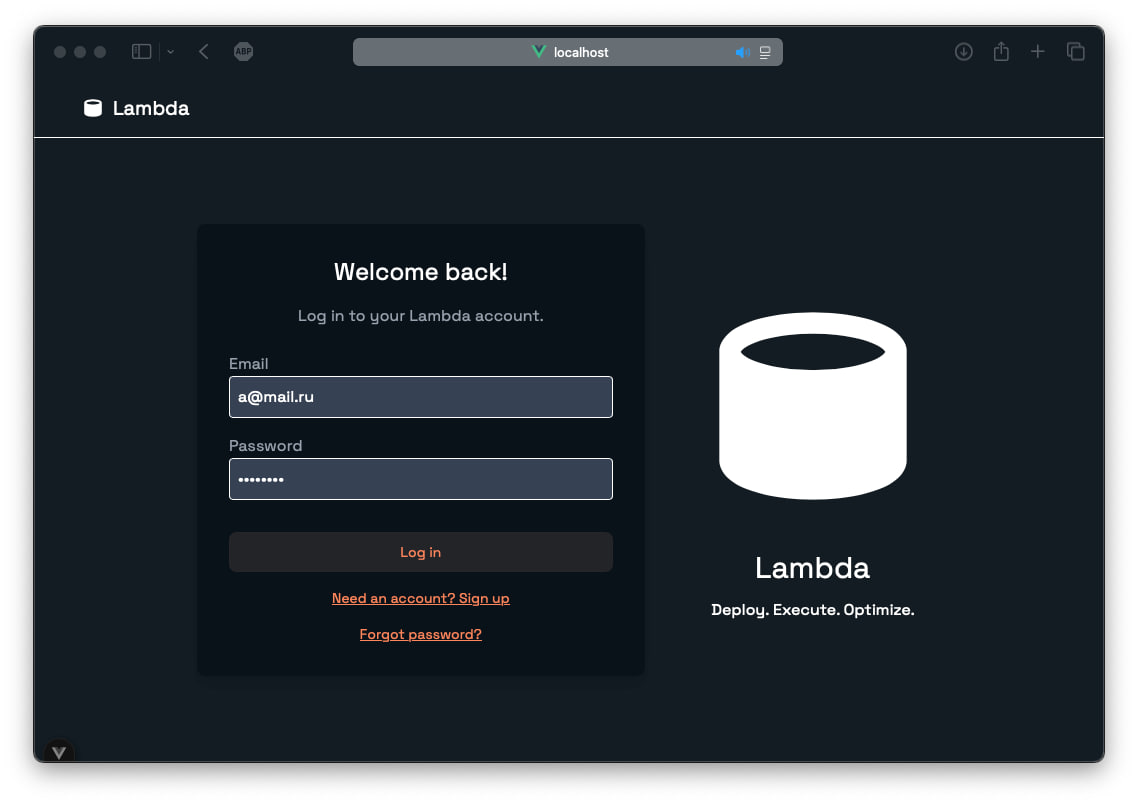
\includegraphics[width=\linewidth]{generated/LoginView.jpg}
  \caption{Форма входа}
  \label{LoginView}
\end{figure*}

Экран входа представлен на рисунке ~\ref{LoginView}, а форма регистрации на рисунке ~\ref{RegistrationView}.

При нажатии кнопки войти или зарегистрироваться, введенные пользователем данные отправляются на соответствующую конечную точку. В случае успешной авторизации полученная пара JWT-токенов сохраняется в сессионное хранилище браузераsessionStorage посредством StorageService. Пользоваетль перенаправляется на стрницу \/tasks.

\begin{figure*}[!t]
  \centering
  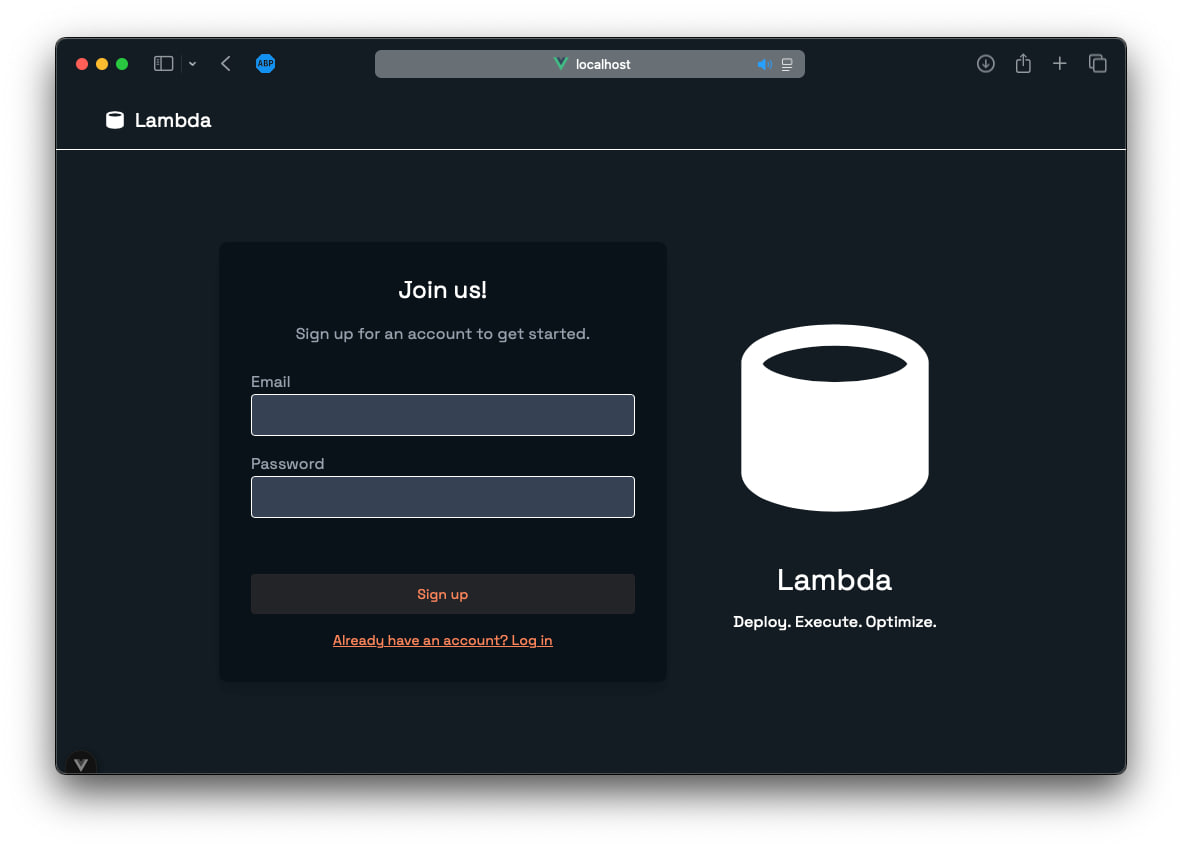
\includegraphics[width=\linewidth]{generated/RegistrationView.jpg}
  \caption{Форма регистрации}
  \label{RegistrationView}
\end{figure*}

В последствии токен досупа пользователя используется при выполнении любых запросов к серверной части платформы. Если время действия токена доступа итекает, сетевой клиент Axios выполнят fallback обработку ошибки 401 полученной от бекенда сервиса и выпускает новый токен досутпа, обращаясь на соответствующий url с токеном refresh\_token, который так же получает из сессионного хранилища.

В случае ошибки, напрмер если пользователем были введены неверные данные или выполнение запроса выло завершщено внутренней ошибкой сервера, информация обошибке, через систему уведомлений выводится на экран пользователя.  Таким образом, система предоставляет пользователю обратную связь и обеспечивает персистентность сессии через StorageService.ts.

\subsubsection{Дашборд Задач}

Основным интерфейсом для взаимодействия пользователя со списком задач является компонент-представление TasksView. При его инициализации (в хуке onMounted)\cite{tikhonova2021design} запускается процесс поллинга задач пользователя через компонет PolligService. Такая реализация позволят своевременно получать изменения статусов задач и получать новые созданные задачи без перезагрузок и каких либо действий со стороны пльзователя.

\begin{figure*}[!t]
  \centering
  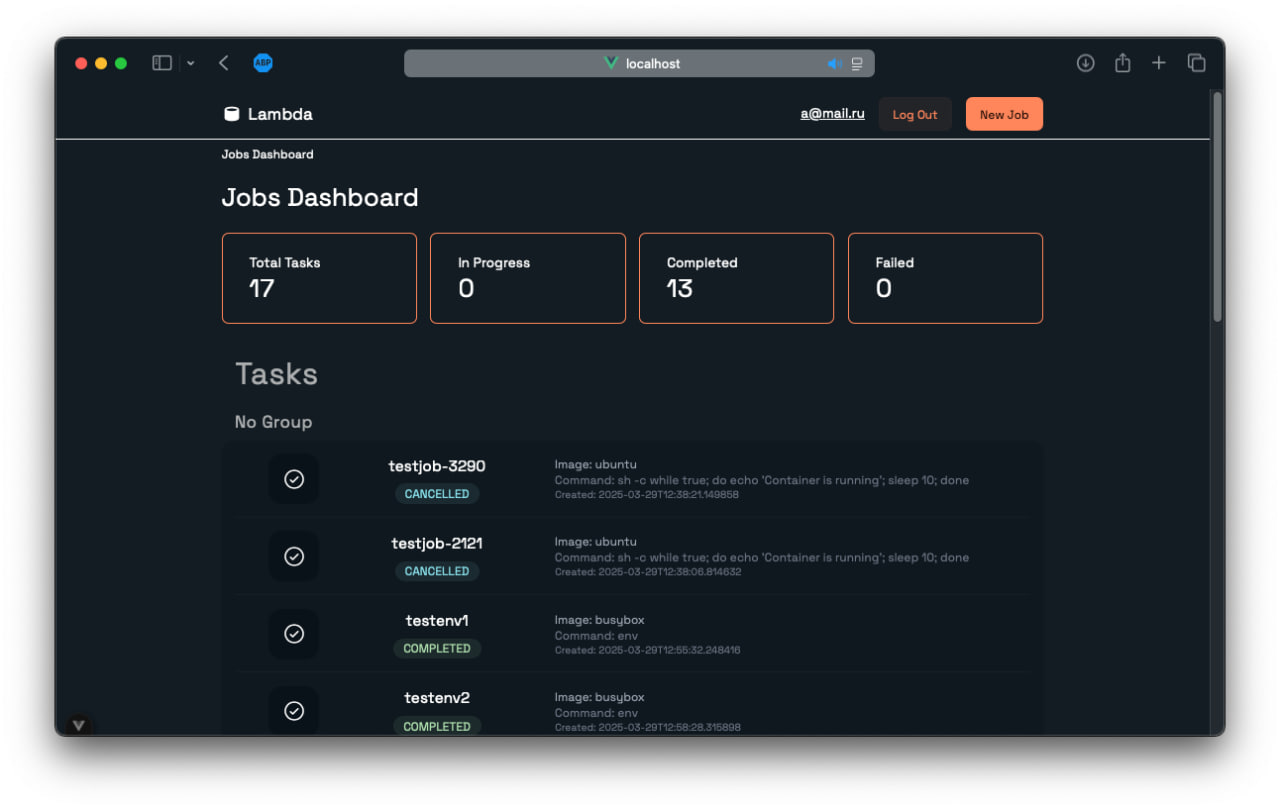
\includegraphics[width=\linewidth]{generated/DashboardView.jpg}
  \caption{Дашборд задач пользователя}
  \label{DashboardView}
\end{figure*}

Дашборд задач представлен на рисунке ~\ref{DashboardView}.

Полученные данные сохраняются в модуле состояния tasksStore.
Компонент TasksView передает этот список задач в дочерний компонент TasksList, который отвечает за их отображение.
TasksList итерируется по списку, для каждой задачи создает экземпляр компонента TaskItem.
Компонент TaskItem отображает ключевую информацию о задаче и использует вложенный компонент StatusBadge для визуализации ее текущего статуса.

\subsubsection{Создание Новой Задачи}

Для создания новых задач предназначена страница CreateJobView, состоящая из формы ввода параметров: имени задачи, типа выполнения (однократный запуск, webhook, cron), Docker-образа, команды и переменных окружения.

Для задач типа CronJob предусмотрено поле ввода Cron-выражения, корректность которого проверяется утилитой CronValidator.ts.

\begin{figure*}[!t]
  \centering
  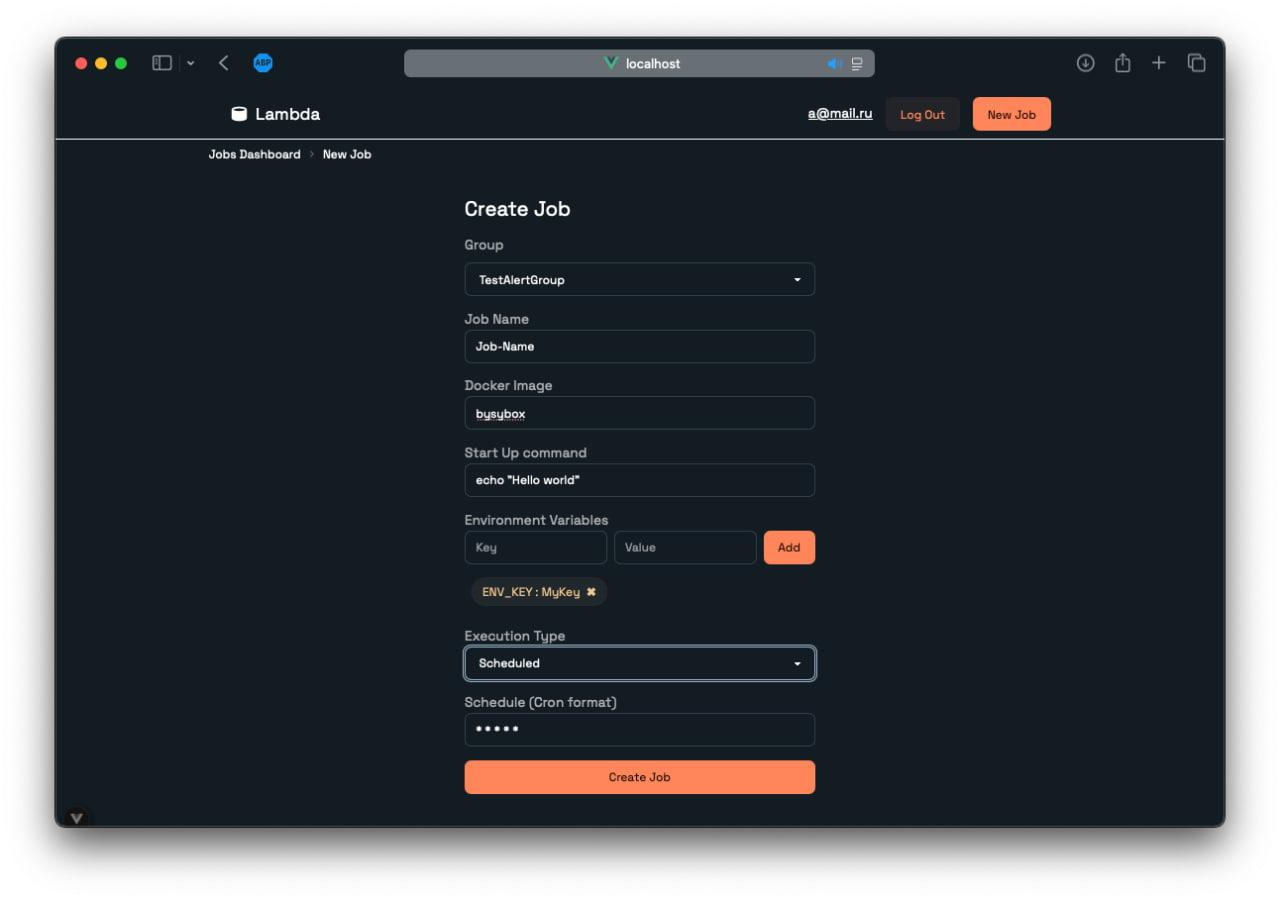
\includegraphics[width=\linewidth]{generated/CreateJobView.jpg}
  \caption{Форма создания новой задачи}
  \label{CreateJobView}
\end{figure*}

Форма содания новой задачи представлена на рисунке ~\ref{CreateJobView}.

После заполнения и клиентской валидации данных формы, CreateJobView инициирует действие выполняет запрос к серверной части приложения с параметрами задачи, заданными пользователем.

При успешном выполнении запроса сервер возвращает подтверждение об усешом создании задачи, пользователю отображается уведомление об успехе через alertStore.showSuccess с последующим перенаправлением на страницу соданной задачи. В случае ошибки API или серверной ошибки, пользователю выводится соответствующее сообщение через alertStore.showError.

\subsubsection{Просмотр Деталей Задачи}

Для отображения подробной информации о конкретной задаче используется страница TaskView(Рис. ~\ref{TaskView}). При переходе по роуту /task/:id компонент извлекает идентификатор задачи из URL. Дальше запускается поллиг сервис задачи, который с определенным интервалом совершает обращения к серверной части платформы для обновления информации по текущей задаче.

\begin{figure*}[!t]
  \centering
  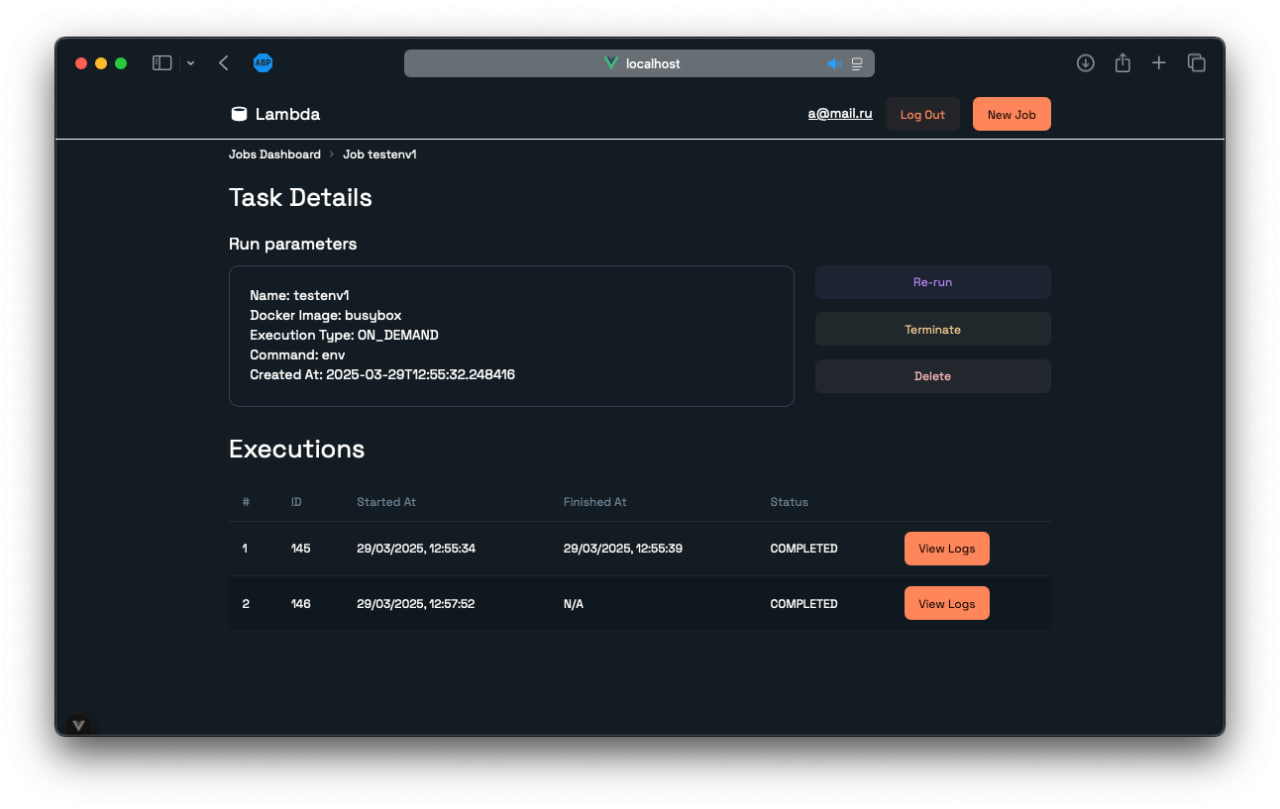
\includegraphics[width=\linewidth]{generated/TaskView.jpg}
  \caption{Экран задачи}
  \label{TaskView}
\end{figure*}

Полученные данные сохраняются в tasksStore и передаются дочерним компонентам: TaskDetails для отображения основной информации о задаче и TaskExecutions для вывода списка ее запусков со статусами и временными метками. При выборе конкретного запуска отображаются его логи в компоненте TaskLogs (Рис. ~\ref{TaskView}).

\begin{figure*}[!t]
  \centering
  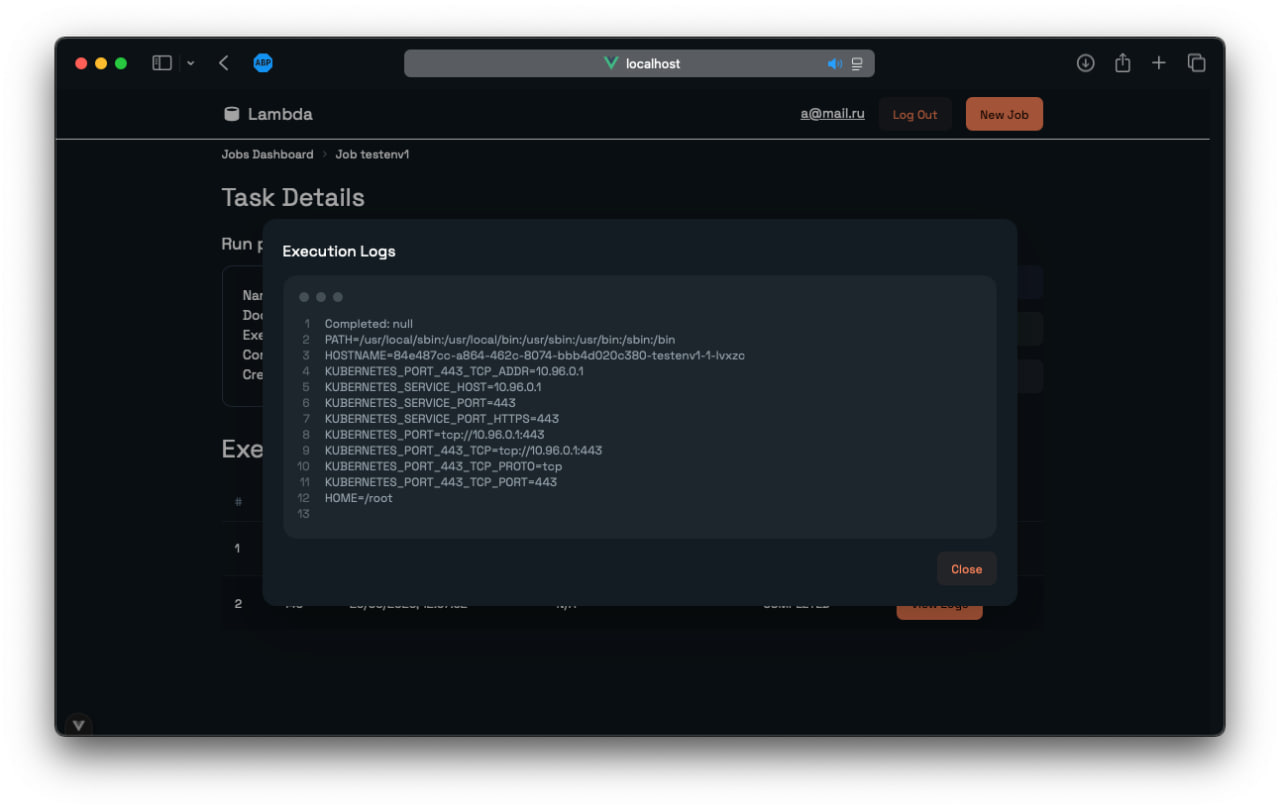
\includegraphics[width=\linewidth]{generated/LogsView.jpg}
  \caption{Модальное окно просмотра логов}
  \label{LogsView}
\end{figure*}

Страница TaskView также предоставляет пользователю возможность выполнять действия над задачей, такие как перезапуск, отмена выполнения, удаление задачи, инициируя соответствующие вызовы API через JobsApi.

\subsubsection{Управление Профилем и Группами}

Раздел ProfileView(Рис ~\ref{TaskView}) предоставляет пользователю инструменты для управления персональными данными и участием в рабочих группах.
При инициализации страницы происходит загрузка информации о текущем пользователе через UserApi.ts с последующим поллингом информации о текущем пользователе и списка групп, в которых он состоит.

\begin{figure*}[!t]
  \centering
  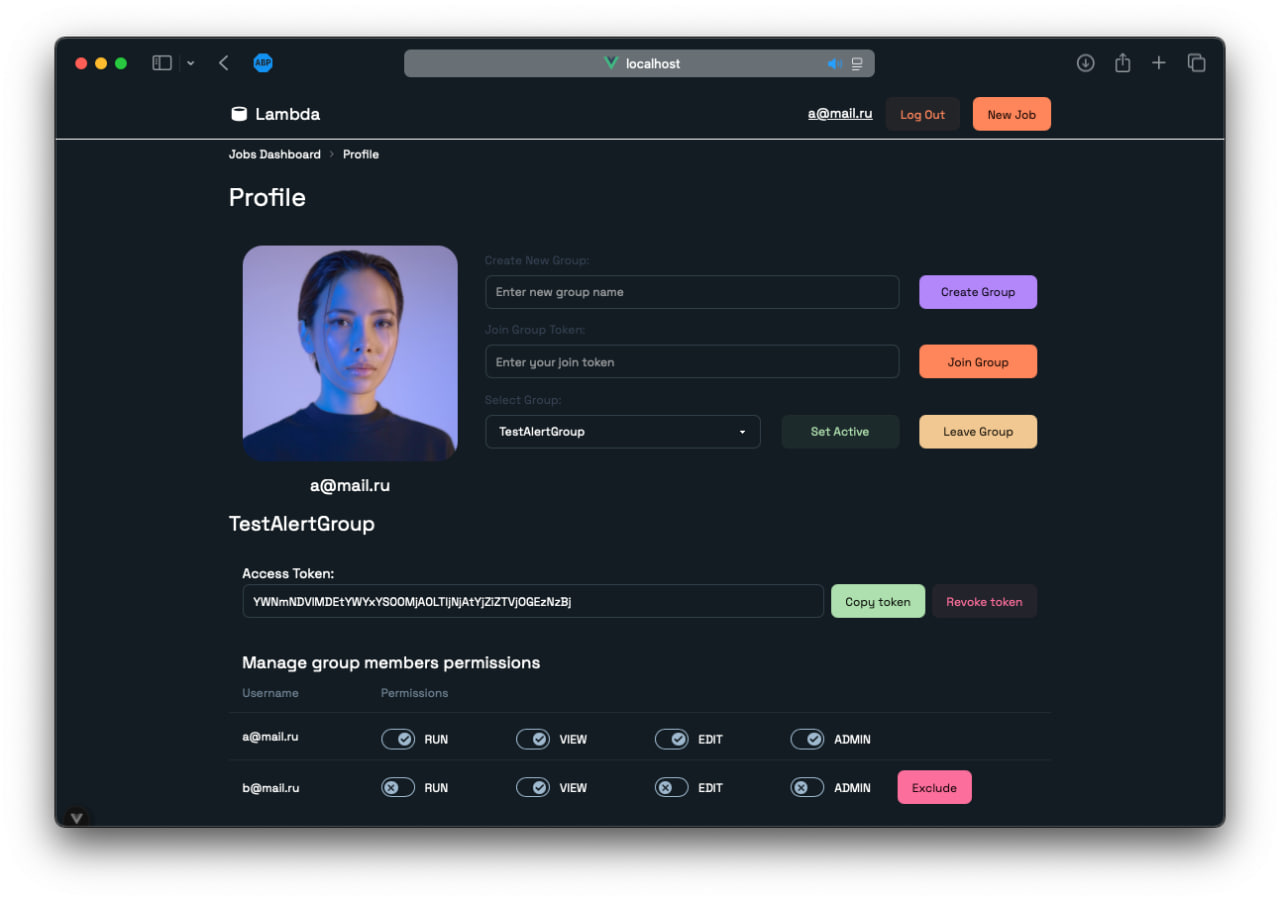
\includegraphics[width=\linewidth]{generated/ProfileView.jpg}
  \caption{Профиль пользователя}
  \label{ProfileView}
\end{figure*}

Данные пользователя отображаются в компоненте ProfileCard.
Список доступных групп представлен в GroupSelection.
Выбор конкретной группы инициирует загрузку списка ее участников и их доступов в рамках группы, которые отображается в MembersTable.
Пользователям с соответствующими правами доступны функции администрирования группы: управление составом и правами доступа участников и генерация токенов приглашения в группу.

Реализованы также механизмы для создания новых групп и присоединения к существующим по токену досутпа.
Управление токенами приглашений осуществляется через компонент AccessToken, который позволяет скопировать действующий токен в буфер обмена или сотозвать действующий токен и сгенерировать новый.

\section{Вывод}

В ходе технической реализации автоматизированной платформа развертывания контейнеризованных функций в среде Kubernetes были применены современные технологии и методы разработки, обеспечивающие эффективность, удобство использования и безопасность системы.

При разработке клиентской части веб-сервиса был использован язык программирования JavaScript с фреймворком Vue.js.  Благодаря исопльзванию соверменных подходов к реализации пользовательского интерфейса обеспечено динамичное взаимодействие с пользователем и удобство в использовании.

Серверная часть платформы разработана с испольванием языка программирования Java и фреймворка Spring Boot для обработки запросов от пользователей, управления данными и взаимодействия с базой данных, сервером авторизации и оркестратором контейнеров.

База данных PostgreSQL использована для хранения информации о пользователях и запущенных задачах. Для работы с учетными записями пользователей использован сервер авторизации Keyloack. Он позволил реализовать авторизацию пользователей с использованием спецификации JWT, а так же предоставил механизмы для реализации гибкой ролевой модедли с динамическим набором групп и доступов.

Для развертывания приложения и обеспечения его доступности и масштабируемости был исопльзован Kubernetes, зарекомендовавший себя как надежное и удобное решение для управления контейнеризованными приложениями.

В результате разработки было создано современное решение, предоставляющее мощный и удобный пользовательский и программный интерфейс для управления распределенными контейнеризованными вычисления. Применение передовых технологий, удобный интерфейс делают этот сервис удобным инструментом для использования в большом колличестве прикладных задач. 